\chapter[The LHC and the ATLAS detector][The LHC and the ATLAS detector]{The LHC and the ATLAS detector}
\label{chap:lhcatlas}

\begin{quote}
  The LHC and ATLAS detector are described.
\end{quote}
 
\section{The LHC}
\label{sec:lhc}

The Large Hadron Collider (LHC)~\cite{cern-jinst-lhc} is the most powerful particle accelerator ever built. It was first conceived in the 1980s with the purpose of finding the Higgs boson and discovering physics beyond our current understanding. It became operation in the early 2010s.

The LHC is a circular hadron collider 27 kilometers in circumference and 100 meters underground, near Geneva, Switzerland. It straddles the border of Switzerland and France. It is operated by the European Organization for Nuclear Research (CERN\footnote{Conseil Europ\'een pour la Recherche Nucl\'eaire}) and occupies the underground tunnel originally constructed for the Large Electron Positron collider (LEP) for use in the 1990s. The construction costs of the LHC are approximately five billion USD.

The LHC collides hadrons at high energies to probe the boundaries of our understanding of particle physics. These collisions are observed by four major experiments situated along the LHC ring: ATLAS~\cite{cern-jinst-atlas}, CMS~\cite{cern-jinst-cms}, ALICE~\cite{cern-jinst-alice}, and LHCb~\cite{cern-jinst-lhcb}. ATLAS and CMS are general purpose particle detector experiments built for discovering physics beyond the Standard Model. ALICE is designed to observe heavy ion (lead nuclei) collisions and study the physics of quark-gluon plasma. LHCb specializes in the study of $b$-hadrons. An aerial view of the experiments is shown in \cref{fig:lhc-switzerland}.

\begin{figure}[tp]
  \centering
  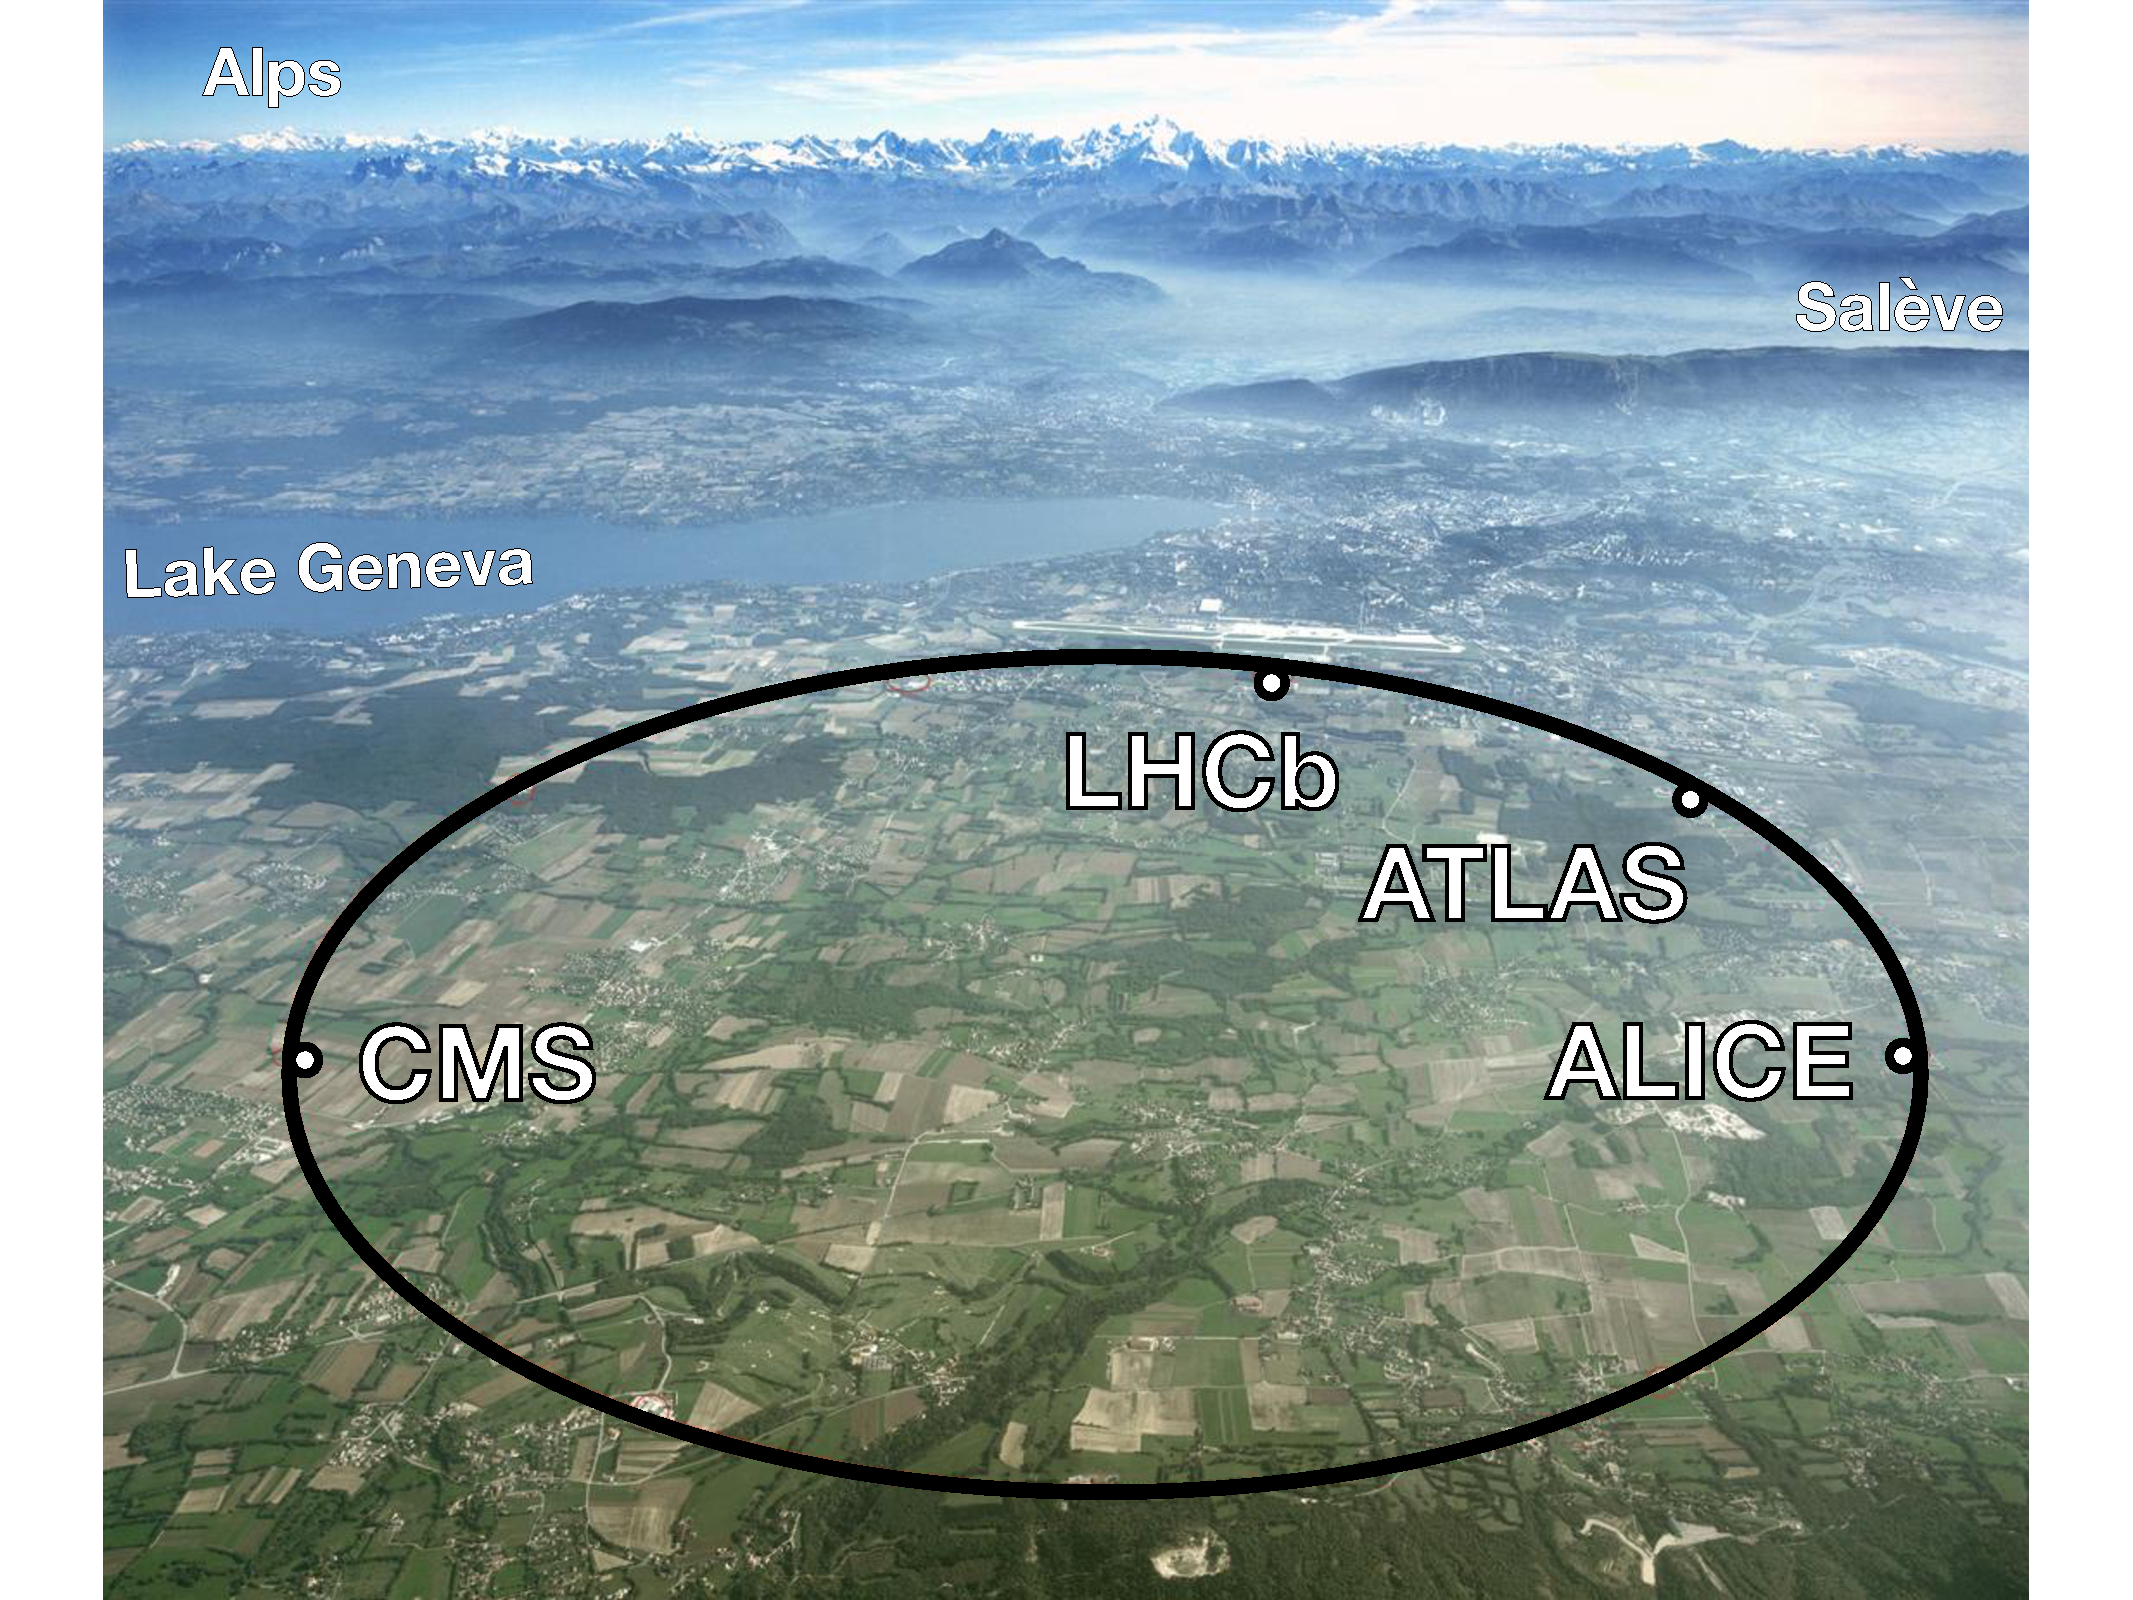
\includegraphics[width=0.90\textwidth]{figures/lhc-atlas/lhc-switzerland}
  \caption{Aerial view of Geneva with an overlaid drawing of the LHC and associated experiments~\cite{atlas-surface}.}
  \label{fig:lhc-switzerland}
\end{figure}

\subsection{Specifications}

The LHC is last step of a multi-stage chain of accelerators called the LHC accelerator complex~\cite{cern-accelerators}, shown in \cref{fig:lhc-complex}. Protons are first retrieved from hydrogen atoms and accelerated by the Linac 2 linear accelerator to 50 MeV per proton. The protons are then passed successively to the Proton Synchotron Booster (PSB), Proton Synchotron (PS), and Super Proton Synchrotron (SPS) where they are accelerated to 1.4 GeV, 25 GeV, and 450 GeV, respectively. The protons are finally fed into the LHC where they are maximally accelerated to 4 TeV in 2012 operations, yielding a center-of-mass collision energy of 8 TeV. This chain is summarized in \cref{tab:experiment-lhc-speeds}. At full energy, the protons will typically circulate the LHC for many hours at a time.

\begin{figure}[tp]
  \centering
  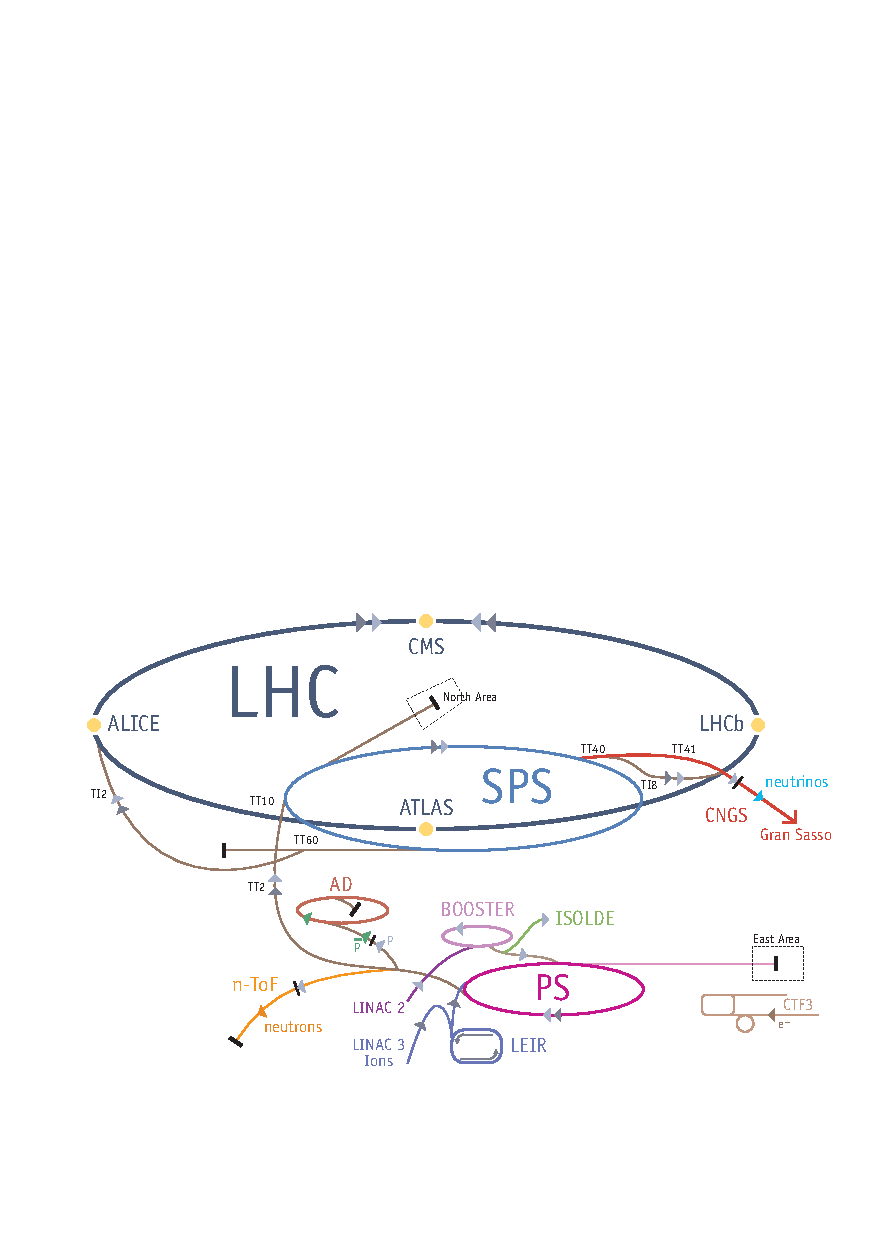
\includegraphics[width=0.90\textwidth]{figures/lhc-atlas/lhc-accelerator-complex}
  \caption{The LHC accelerator complex. Before reaching the LHC, protons are accelerated at Linac 2, the Proton Synchrotron Booster (PSB), the Proton Synchrotron (PS), and the Super Proton Synchrotron (SPS)~\cite{cern-faq}.}
  \label{fig:lhc-complex}
\end{figure}

\begin{table}[bp]
  \centering
  \renewcommand{\arraystretch}{1.4}
  \caption{The accelerators of the LHC accelerator chain and the speed at which they accelerate protons in 2012.~\cite{cern-faq}.}
  \begin{tabular}{c|c|c}
  proton energy (GeV) & speed of light (\%) & accelerator \\
  \hline
     0.05             & 31.4                & Linac 2     \\
     1.4              & 91.6                & PSB         \\
    25                & 99.93               & PS          \\
   450                & 99.9998             & SPS         \\
  4000                & 99.999997           & LHC         \\
\end{tabular}


  \label{tab:experiment-lhc-speeds}
\end{table}

Protons travel around the LHC in two oppositely circulated beams. The proton beams are bent and focused by powerful superconducting electromagnets, which operate cryogenically at an ultracold temperature of 2 K (-456 F). The proton beams are segmented into groups of protons called \textit{bunches}. Each beam contains 2808 bunches, and each bunch contains approximately $10^{11}$ protons. Many protons are included per bunch to maximize the probability of a proton-proton collision for a given bunch crossing. A bunch crossing happens every 50 nanoseconds during operations in 2012.

\subsection{Operations}

The LHC is designed to collide protons with a center-of-mass energy $\sqrt s$ of 14 TeV and an instantaneous luminosity of $10^{34}\lumi$. However, while commissioning in 2008, the machine broke due to a faulty electrical connection between two superconducting magnets~\cite{cern-incident}. The LHC was repaired in 2009 and, to ensure safer operation, began colliding protons below design energy and instantaneous luminosity in late 2009.

The LHC collided protons for physics studies in 2010-2012 at a reduced energy of 7 TeV (2010-2011) and 8 TeV (2012). These years of data-taking are referred to as \textit{Run-I} and include the discovery of the Higgs boson. The peak instantaneous luminosity achieved was $7.7 \times 10^{33}\lumi$ in 2012~\cite{cern-run1}, which more than doubled the peak luminosity of 2011 data-taking. 

To increase the number of collisions recorded, many proton collisions are allowed to occur within a single bunch crossing. This average number of proton collisions per bunch crossing $\pileup$ is referred to as \textit{pileup}. The average $\pileup$ in 2012 is around 20 collisions per crossing and reaches as large as 35-40. Profiles of the pileup are shown in \cref{fig:atlas-lumi-1,fig:atlas-lumi-2}.

\begin{figure}[tp]
  \centering
  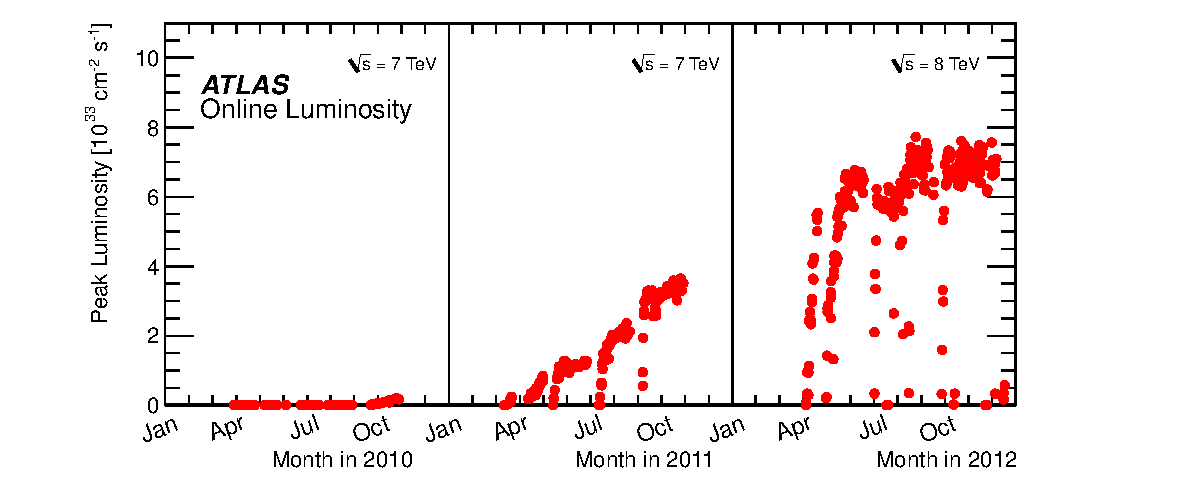
\includegraphics[width=0.90\textwidth]{figures/lhc-atlas/lumivstime}
  \caption{The peak luminosity as measured in different data-taking periods~\cite{atlas-lumi}. The peak Run-I luminosity is $0.8\times 10^{34} \text{cm}^{-2} \text{s}^{-1}$.}
  \label{fig:atlas-lumi-1}
\end{figure}

\begin{figure}[tp]
  \centering
  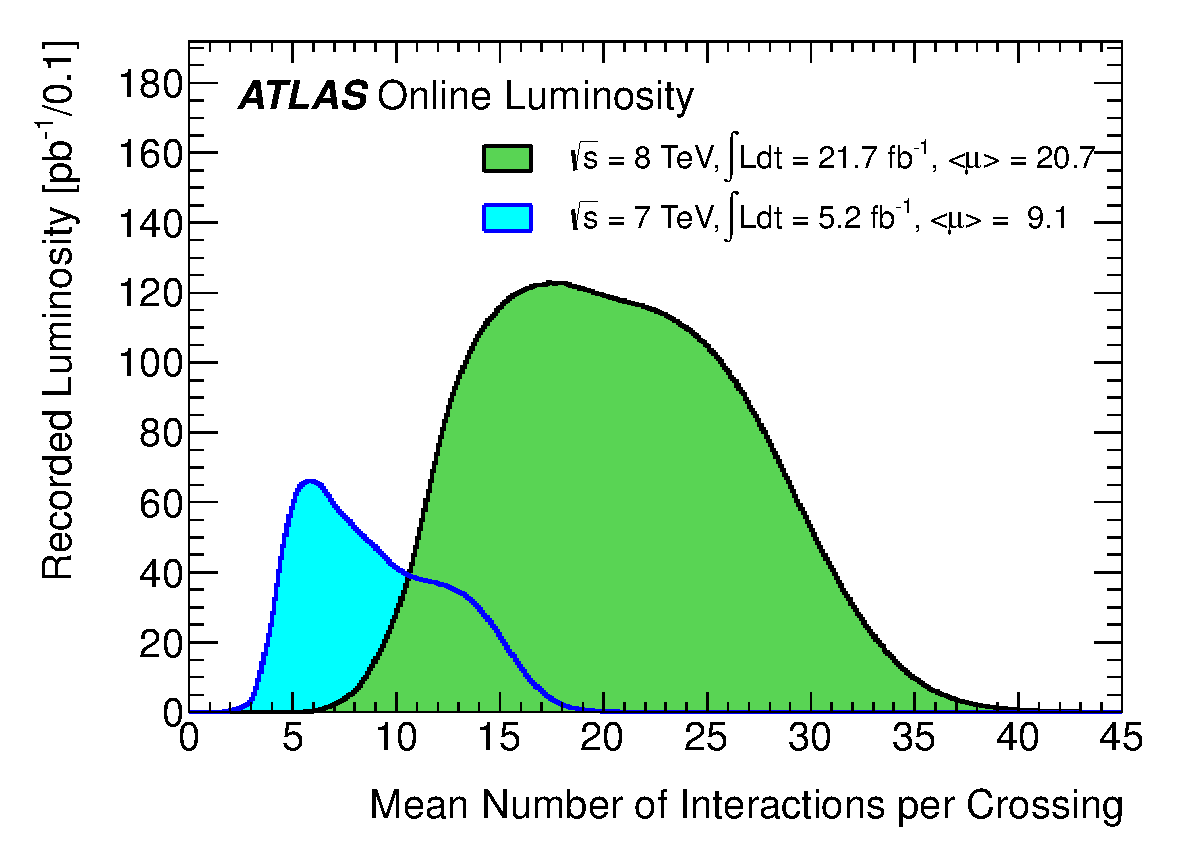
\includegraphics[width=0.48\textwidth]{figures/lhc-atlas/mu_2011_2012-dec}
  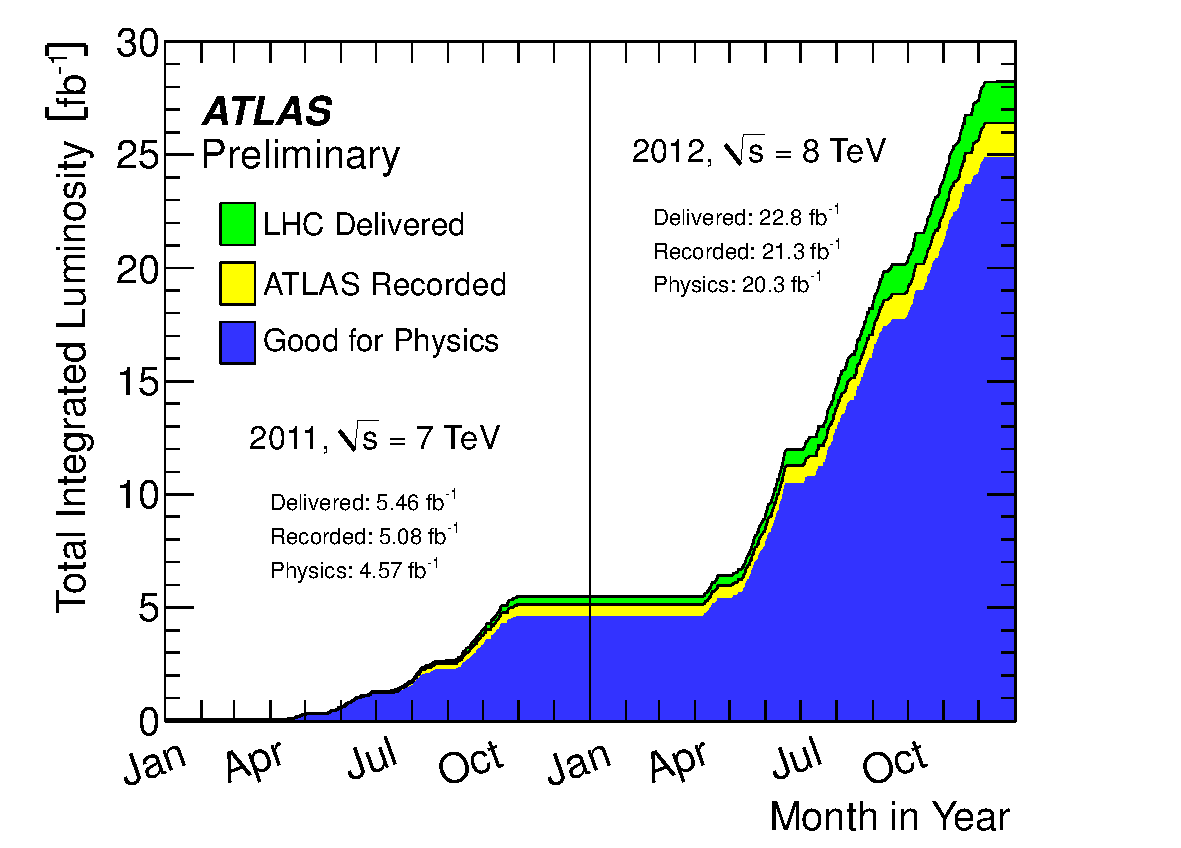
\includegraphics[width=0.48\textwidth]{figures/lhc-atlas/intlumivstime2011-2012DQ}
  \caption{Distributions of the recorded luminosity in bins of $\pileup$ (left) and the total integrated luminosity as a function of time (right)~\cite{atlas-lumi}. In 2011 (2012), the average $\pileup$ is 9.1 (20.7) and the total integrated luminosity for physics analysis is 4.6 $\ifb$. (20.3 $\ifb$).}
  \label{fig:atlas-lumi-2}
\end{figure}

The LHC, ATLAS, and CMS are undergoing maintenance and upgrades from early 2013 until early 2015. Data-taking is intended to resume in mid-2015 with an increased $\sqrt{s}=13$ TeV and a instantaneous luminosity of $10^{34}\lumi$. The \textit{Run-II} data-taking campaign is intended to last for the next three to four years, until 2017-2018, when another round of upgrades are planned to be installed.

These datasets allow the ATLAS and CMS experiments to probe physics of the Standard Model and beyond unlike any previous experiment in particle physics. Despite operating below design energy and luminosity, the Run-I dataset accesses electroweak processes at unprecedented rates, as shown in \cref{fig:lhc-stirling}. This rate will increase again in the Run-II data-taking campaign, thereby offering a new opportunity for discovery.

\begin{figure}[tp]
  \centering
  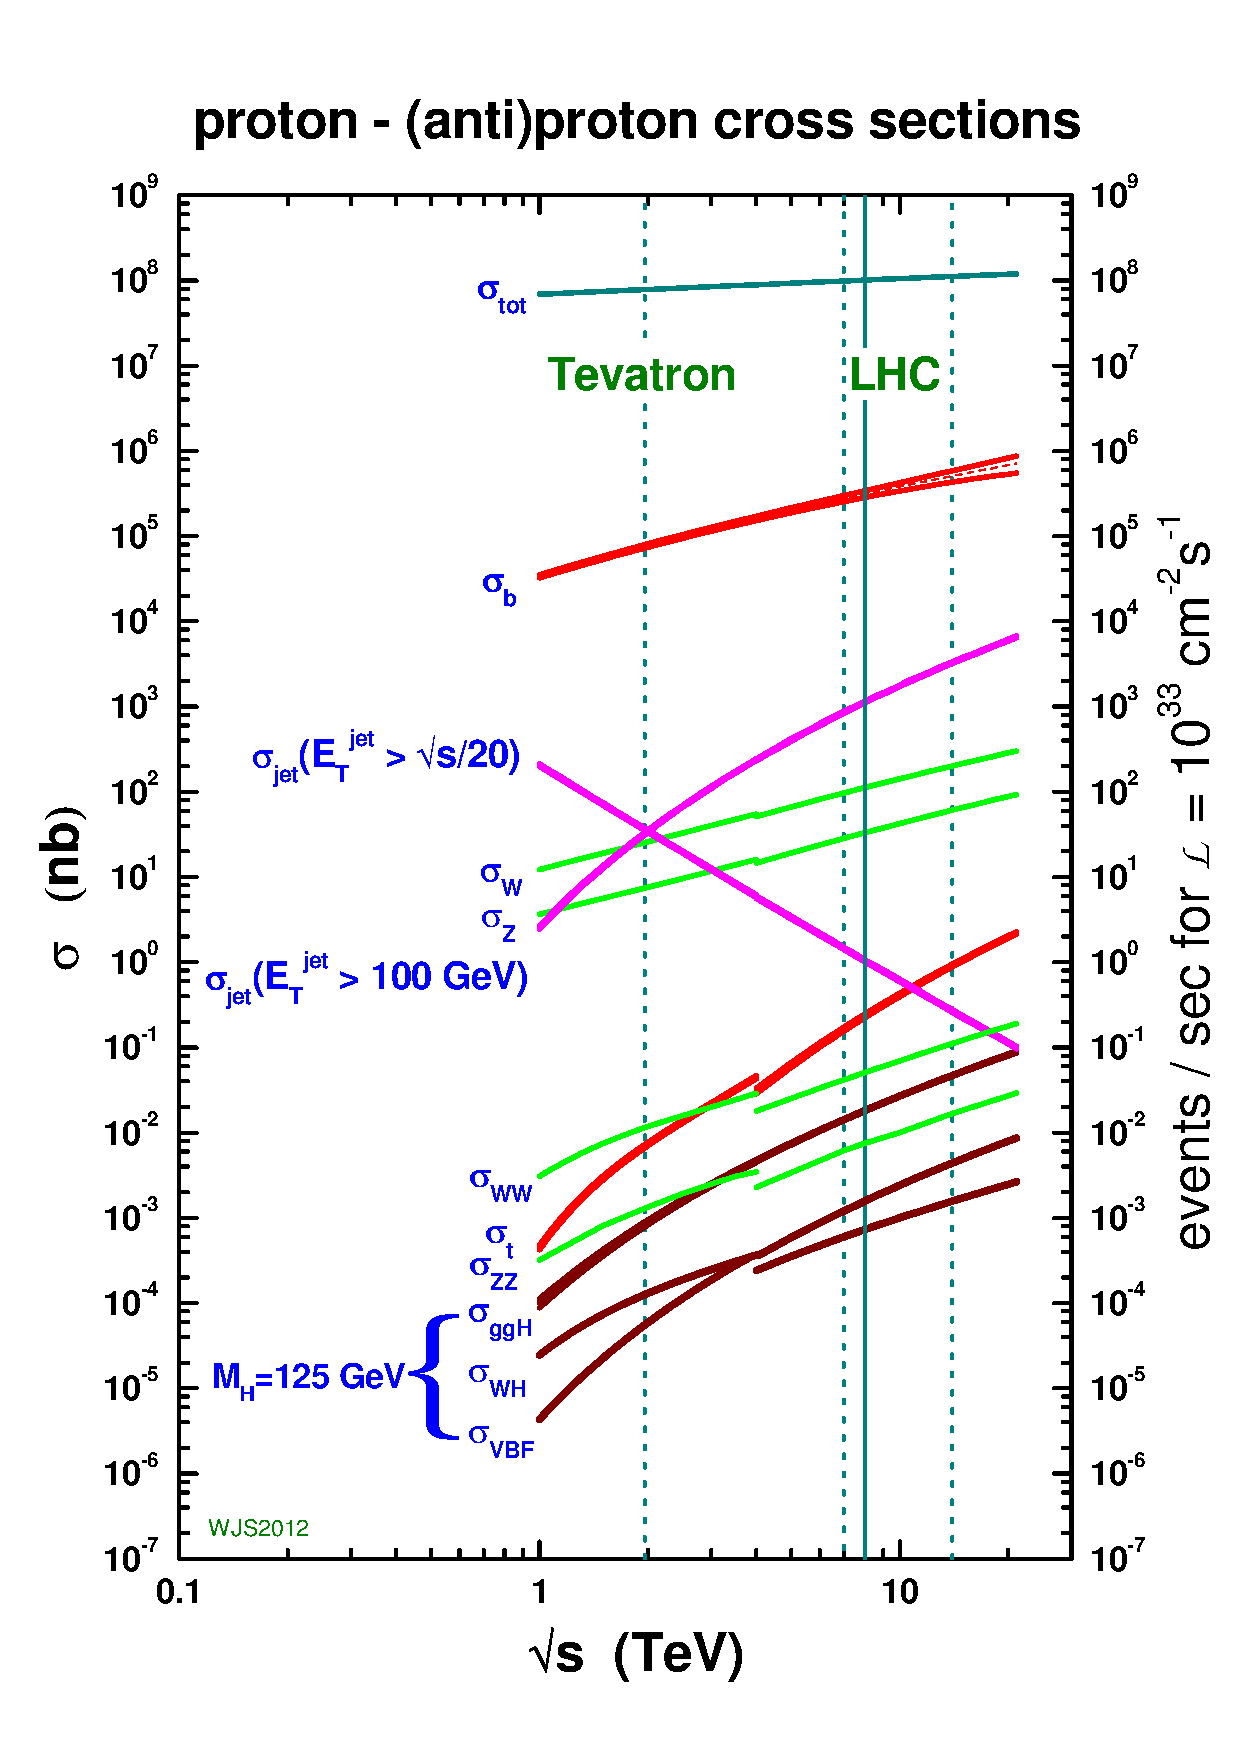
\includegraphics[width=0.90\textwidth]{figures/lhc-atlas/crosssections2012_v5}
  \caption{Cross sections for $pp$ and $p\overline{p}$ processes in the center-of-mass energy regime relevant to the Tevatron and LHC, courtesy of W.J. Stirling~\cite{2013.stirling.cross-sections}.}
  \label{fig:lhc-stirling}
\end{figure}

\section{The ATLAS detector}
\label{sec:atlas}

The ATLAS\footnote{\textbf{A} \textbf{T}oroidal \textbf{L}HC \textbf{A}pparatu\textbf{s}} detector is a general purpose cylindrical detector centered on one of the LHC collision points. It is 46 meters in length, 25 meters in diameter, and weighs 7000 tons. Assembly began at CERN in 2003 and construction was completed in 2008. A schematic rending is shown in \cref{fig:atlas-cartoon}.

\begin{figure}[tp]
  \centering
  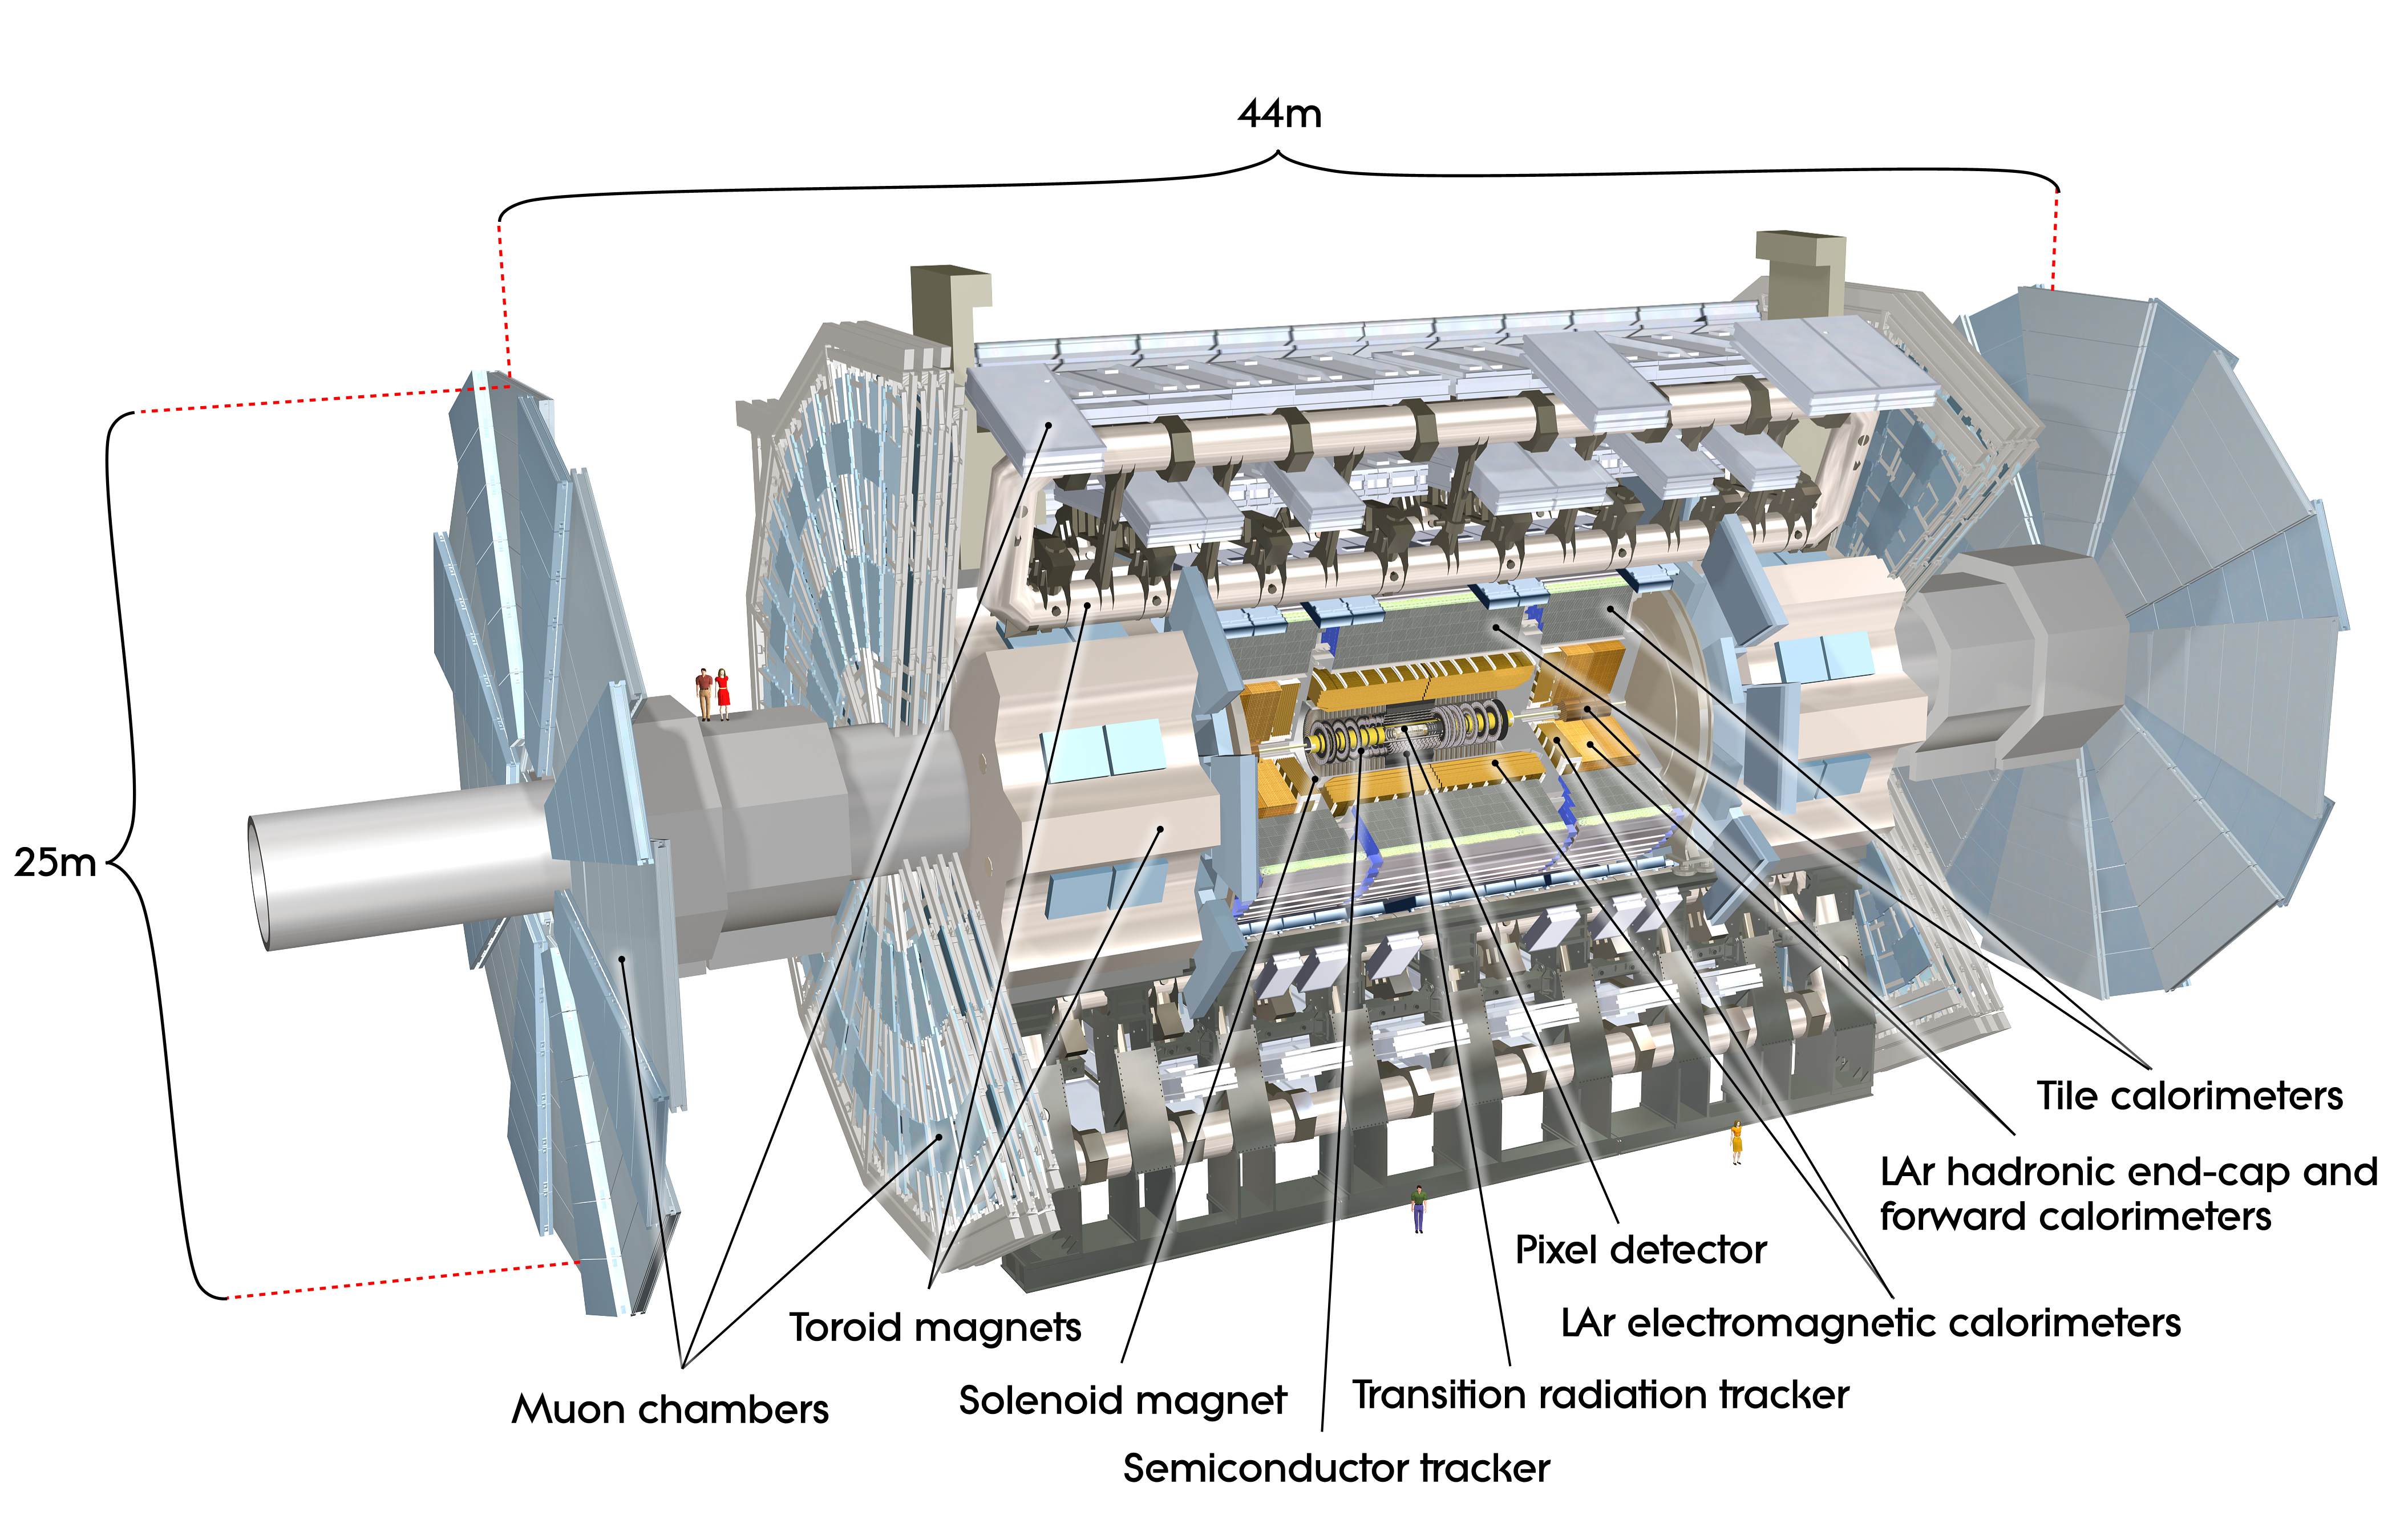
\includegraphics[width=0.90\textwidth]{figures/lhc-atlas/atlas-0803012_01.jpg}
  \caption{Scale rendering of the ATLAS detector with the various subdetectors highlighted~\cite{atlas-cgi-detector}.}
  \label{fig:atlas-cartoon}
\end{figure}

ATLAS is built to measure and classify particles arising from proton-proton collisions. These particles can be as low energy as a few hundred MeV to as high energy as multiple TeV. To detector such a broad range of phenomena, multiple subdetectors are employed. These are concentric about the proton-proton interaction point (IP) and are designed to observe different classes of particles. 

The \textit{inner detector} is closest to the beams and is designed to detect charged particles. The \textit{calorimeters} are outside the inner detector and are designed to stop all particles except muons and neutrinos. The \textit{muon system} is furthest from the beams and is designed to detect muons as they exit ATLAS. 

The inner detector is enclosed by a solenoidal magnet with a field of approximately 2 Tesla. A large toroidal magnet exists within the muon system which has a field of approximately 4 Tesla. The purpose of these magnets is to bend the trajectory of charged particles as they travel through ATLAS. The momenta of these particles can then be precisely inferred from the measured trajectory according to the classical Lorentz force law.

ATLAS uses a right-handed coordinate system with its origin at the IP in the center of the detector, and the $z$-axis along the beam line. The $x$-axis points from the IP to the center of the LHC ring, and the $y$-axis points upwards. Cylindrical coordinates ($r$, $\phi$) are used in the transverse plane, $\phi$ being the azimuthal angle around the beam line. The pseudorapidity $\eta$ is typically used in place of the polar angle $\theta$ and is defined as $\eta = -\text{ln}(\text{tan}\frac{\theta}{2})$~\cite{HIGG-2012-27}.

The ATLAS collaboration was formed in 1992, and as of 2011, it includes over 3000 scientists from 174 institutions and 38 countries. It is one of the largest scientific collaborations in the world.

\begin{figure}[tp]
  \centering
  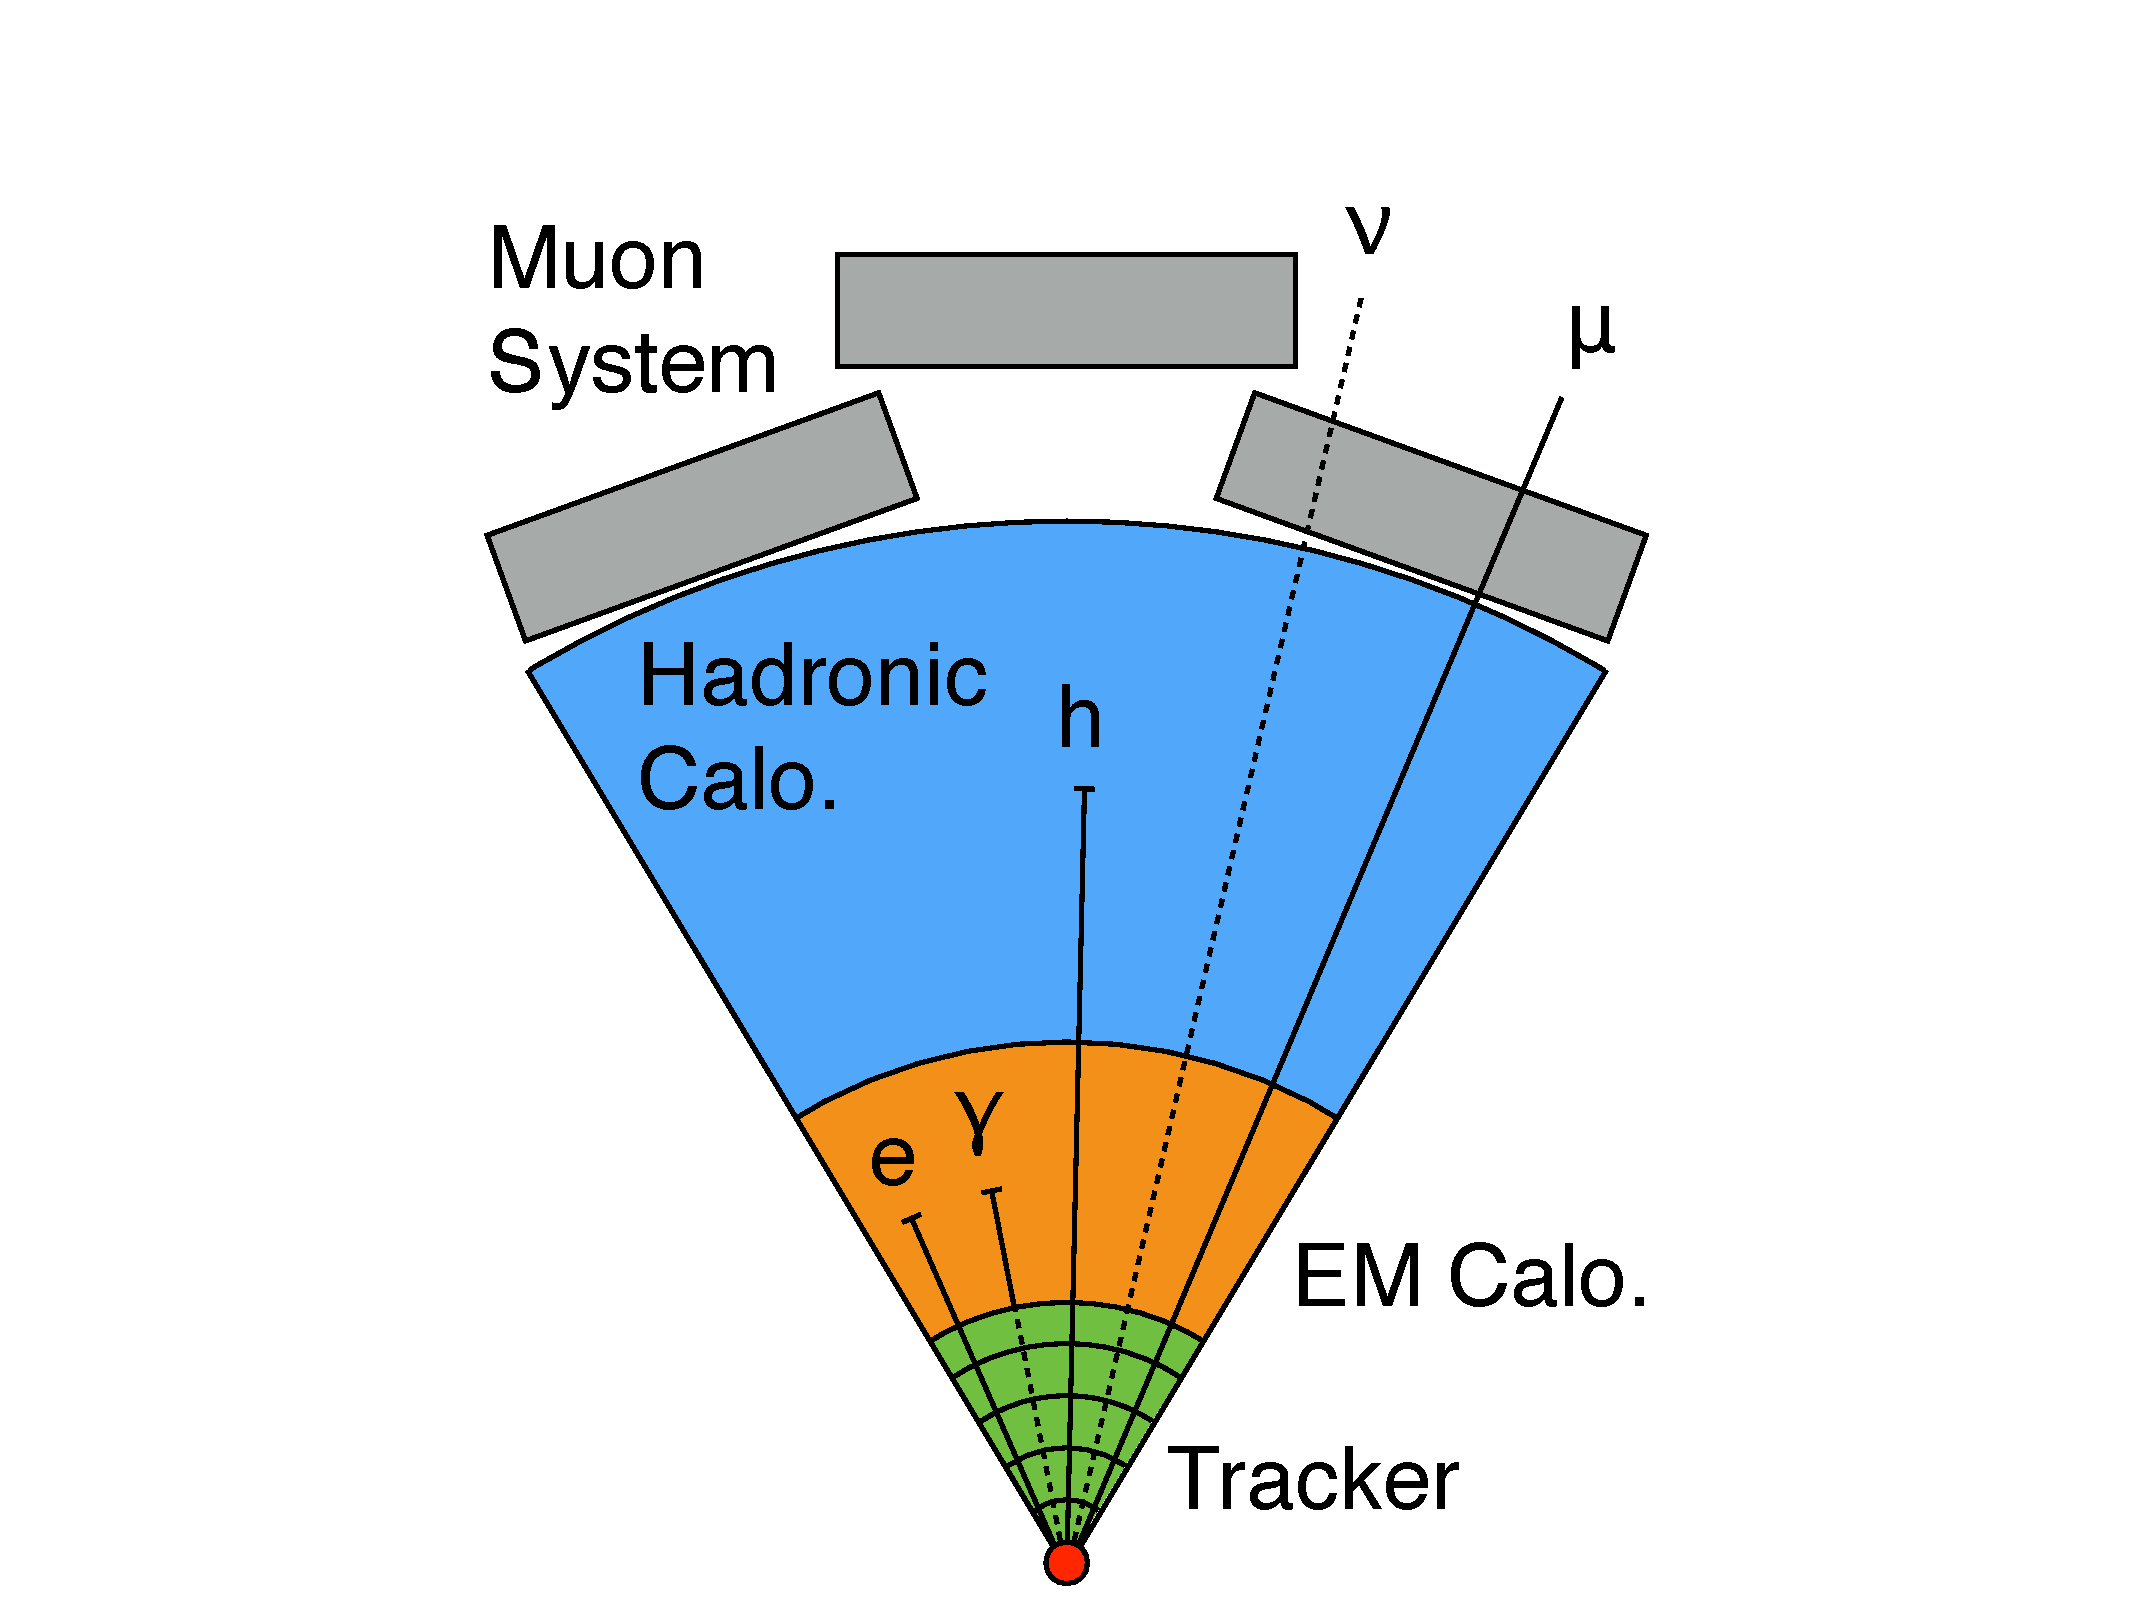
\includegraphics[width=0.5\textwidth]{figures/lhc-atlas/atlas-wedge-cartoon}
  \caption{Transverse schematic view of a wedge of the ATLAS detector. Charged particles leave tracks in the tracker, electrons and photons typically stop in the electromagnetic calorimeter, hadrons like charged pions typically stop in the hadronic calorimeter, and muons are tagged by the muon system as they exit. Neutrinos escape undetected.}
  \label{fig:atlas-wedge}
\end{figure}

\subsection{Inner detector and tracking}

The inner detector (ID), also called the \textit{tracker}, is designed to precisely measure the trajectory and momentum of charged particles as they pass through the 2 T magnetic field provided by the solenoid, such as electrons, muons, and charged pions~\cite{cern-jinst-atlas}. The ID is composed of three independent but complementary subdetectors: the Pixel detector, the Semiconductor Tracker (\textit{SCT}), and the Transition Radiation Tracker (\textit{TRT}). These are shown in \cref{fig:atlas-detector-id}. The subdetectors are split into barrel and endcap components, have full $2\pi$ coverage in $\phi$, and have at least coverage in $|\eta|$ up to 2.0. Information from all subdetectors is used to reconstruct tracks and vertices.

\begin{figure}[tp]
  \centering
  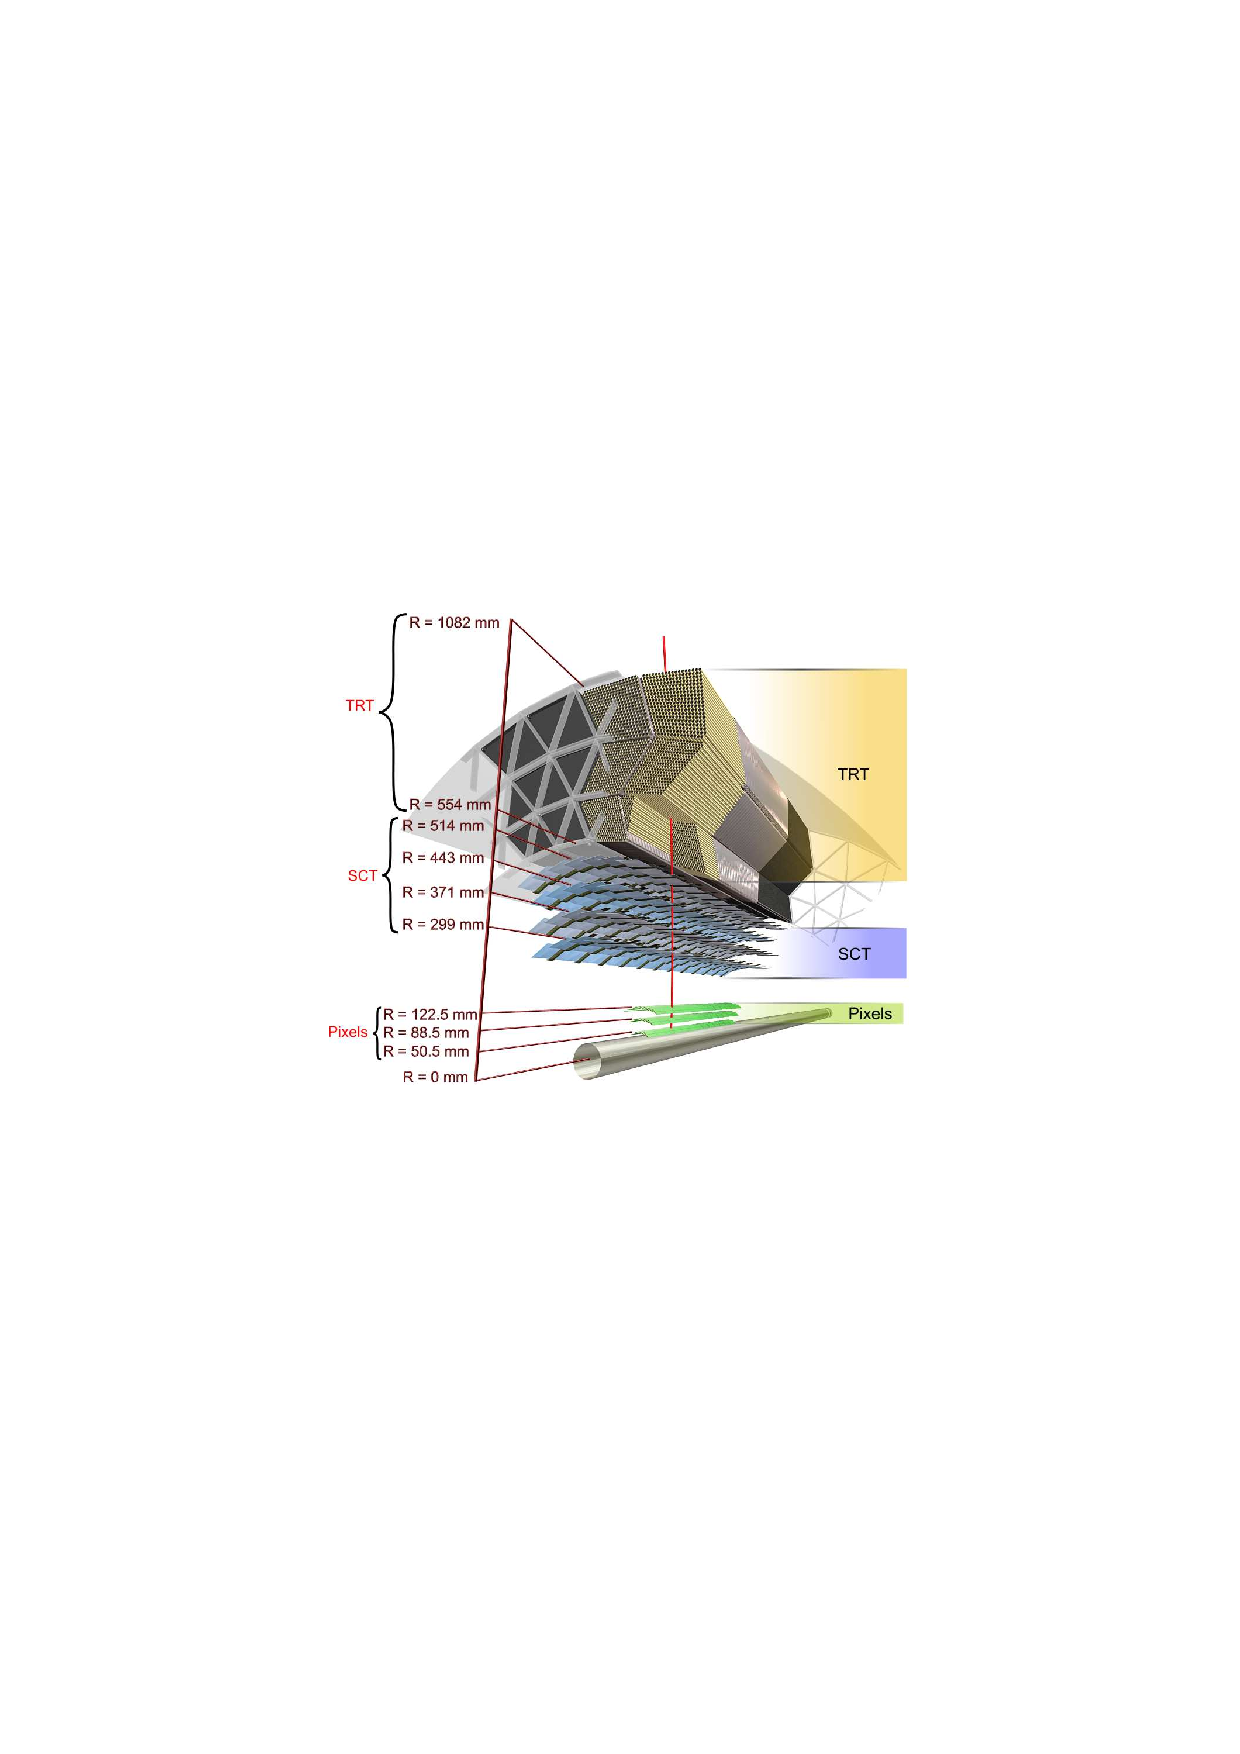
\includegraphics[width=0.7\textwidth]{figures/lhc-atlas/detector-ID}
  \caption{A diagram of the barrel of the Inner Detector: the three layers in the Pixels, the four layers in the SCT, and the many layers of the TRT~\cite{ATLAS-CONF-2014-047}.}
  \label{fig:atlas-detector-id}
\end{figure}

\subsubsection{Subdetectors}

The Pixel detector exists closest to the interaction point and employs three layers silicon pixels~\cite{cern-jinst-atlas}. The pixels have fine granularity and are designed to deliver precise measurement of tracking parameters close to the IP, which are useful for secondary vertexing. The intrinsic resolution of the pixels in the barrel are $10\ \micron$ in $r\phi$ and $115\ \micron$ in $z$. The Pixel detector has 80 $\times 10^{6}$ channels, by far the most of any ATLAS subdetector, and usually provides three measurements per charged particle. The track resolution is $10\ \micron$ The Pixel detector has coverage up to $|\eta|=2.5$.

The SCT surrounds the Pixel detector and also employs silicon detector elements, using micro-strips instead of pixels~\cite{cern-jinst-atlas}. The strips are arranged in four double layers, with the the pairs arranged at small angles relative to each other, to make a three-dimensional measurement. The intrinsic resolution of the strips in the barrel are $17\ \micron$ in $r\phi$ and $580\ \micron$ in $z$. The SCT has 6.3 $\times 10^{6}$ channels and usually provides eight measurements per charged particle. It has coverage up to $|\eta|=2.5$.

The TRT surrounds the SCT and is the largest of the ID subdetectors~\cite{cern-jinst-atlas}. It employs 300,000 straw drift tubes for recording the passage of charged particles. The intrinsic resolution of the TRT in the barrel is $130\ \micron$ in $r\phi$; the drift tubes cannot make a measurement in $z$. The TRT has 350,000 channels and usually provides 30 or more measurements per charged particle. It has coverage up to $|\eta|=2.0$. A comparison of subdetector features is shown in \cref{tab:experiment-atlas-id}.

\begin{table}[bp]
  \centering
  \renewcommand{\arraystretch}{1.2}
  \caption{Features of the subdetectors in the barrel of the Inner Detector: the Pixel detector, the SCT, and the TRT~\cite{ATLAS-CONF-2014-047}.}
  \begin{tabular}{c|cccccc}
  Subdetector & Channels           & Element size [$\micron$] & Resolution [$\micron$] & Layer radii [mm]   \\
  \hline
  Pixels      & 80$\times 10^{6}$  & $50 \times 400$          & $10 \times 115$        & 50.5, 88.5, 122.5  \\
  SCT         & 6.3$\times 10^{6}$ & $80 \times 120000$       & $17 \times 580$        & 299, 371, 443, 514 \\
  TRT         & 350$\times 10^{3}$ & $4000$                   & $130 \times \emptyset$ & 554 -- 1082        \\
\end{tabular}


  \label{tab:experiment-atlas-id}
\end{table}

The TRT additionally provides information for classifying charged particles as electrons or pions via the detection of transition radiation in the xenon gas mixture in the drift tubes~\cite{ATLAS-CONF-2011-128}. This radiation is produced when a charged particle crosses the boundary between two media of different dielectric constants (polypropylene) and is proportional to the Lorentz $\gamma$ of a particle. For an electron and charged pion of equal momentum, the electron is therefore much more likely to produce TR than the pion since its mass is 200 times smaller.

\subsubsection{Tracking}

Information from these three subdetectors are combined to make \textit{tracks}, which have a unique correspondence to charged particles and are meant to describe their trajectory and momentum. As a charged particle travels through the ID, it leaves \textit{hits} in each subdetector along its trajectory. These are built into tracks with a three-dimensional fit using Kalman filtering tools which can account for scattering as the charged particle traverses the media of the ID~\cite{ATLAS-CONF-2014-047,ATLAS-CONF-2012-042}. The ATLAS tracking algorithms builds tracks for charged particles as low momentum as a few hundred MeV.

A vertex reconstruction algorithm~\cite{ATLAS-CONF-2010-069,ATLAS-CONF-2012-042} is used to determine if multiple tracks originate from a single $pp$ collision. The output of the algorithm is a complete set of vertices per event and the association of each track to a vertex. Starting with the set of all tracks passing simple goodness criteria (e.g., requiring a minimum number of hits in the silicon detectors), a vertex seed is derived from the global maximum of $z$ coordinates, and tracks are associated to that seed using a $\chi^2$ fitting algorithm. Tracks incompatible with the vertex are then used as seeds for the next iteration of the vertexing algorithm until all tracks are exhausted. 

Vertexing is essential for deciding which tracks (and thus physics objects) originate from the $pp$ collision of interest and which tracks do not. The vertex associated to the collision of interest is called the \textit{primary vertex} and is conventionally the vertex with the highest $\sumtrackpt$ associated to it. If a track is not consistent with having been produced in the primary vertex, it is typically ignored as originating from a pileup interaction which is uninteresting. This is the best and most intuitive method of ignoring pileup contributions since the calorimeter cannot extrapolate particle trajectories back to the beamline with nearly as good precision. A visualization of the power of tracking for pileup rejection is shown in \cref{fig:atlas-detector-pileup}.

\begin{figure}[tp]
  \centering
  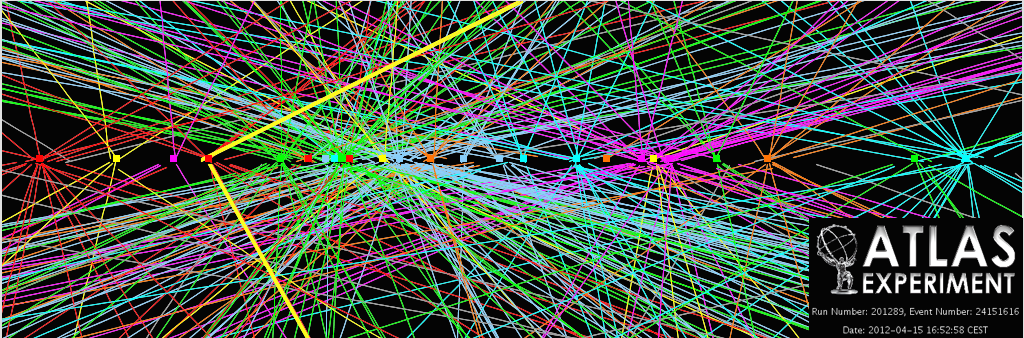
\includegraphics[width=0.95\textwidth]{figures/lhc-atlas/2012_highPileup.png}
  \caption{Event display of a $\Zmumu$ event with 25 reconstructed vertices in 2012 data-taking~\cite{atlas-eventdisplays}.}
  \label{fig:atlas-detector-pileup}
\end{figure}

A track can then be described by five parameters: the transverse impact parameter relative to the primary vertex $d_0$, the longitudinal impact parameter $z_0$, the azimuthal angle $\phi_0$, the polar angle $\theta$, and the ratio of charge to momentum $q/p$. 

\subsection{Calorimeters and clustering}

The ATLAS calorimeters sit outside the inner detector and the solenoid magnet. They are designed to stop particles like electrons, photons, and pions and to measure their energy. The calorimeters are grouped into electromagnetic (EM) and hadronic calorimeters, where the name describes the class of particle they are designed to stop. Both classes of calorimeters are \textit{sampling} calorimeters, meaning only a fraction of a particle shower energy is observed, and the full shower energy must be inferred. Dense absorber material is used to initiate showers, and interleaved active material is used for detecting the showers.

The calorimeter subdetectors are shown in \cref{fig:atlas-detector-calorimeters}. They are split into barrel and endcap components, have full $2\pi$ coverage in $\phi$, and have coverage in $|\eta|$ up to 4.9. Information from all subdetectors is used to reconstruct calorimeter clusters.

\begin{figure}[tp]
  \centering
  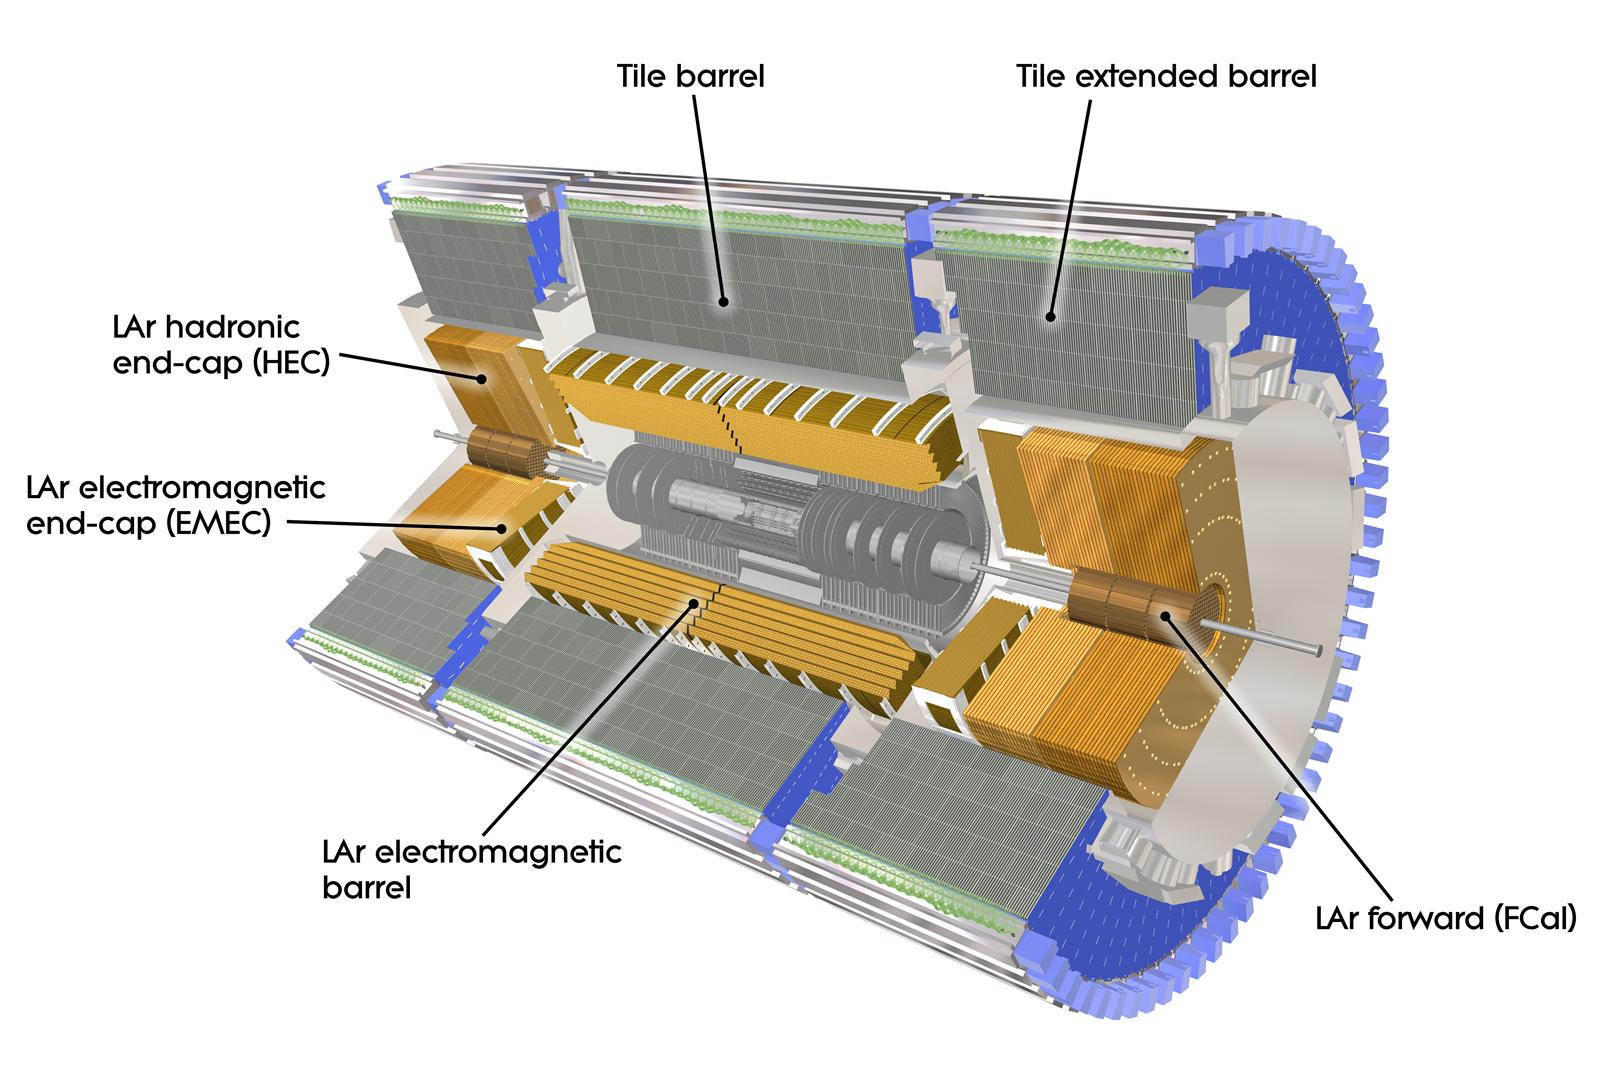
\includegraphics[width=0.95\textwidth]{figures/lhc-atlas/detector-calorimeters}
  \caption{A diagram of the ATLAS calorimeters~\cite{cern-jinst-atlas}.}
  \label{fig:atlas-detector-calorimeters}
\end{figure}

\subsubsection{Subdetectors}

The EM calorimeters are subdivided into barrel and endcap components, which cover $|\eta| < 1.5$ and $1.4 < |\eta| < 3.2$. An additional presampler exists for $|\eta| < 1.8$ to account for showers starting before the calorimeter. Lead plates are used as the absorber material with liquid argon (LAr) as the active material. An accordion-style geometry is employed for uniform $\phi$ coverage without azimuthal cracks. The EM calorimeter is radially subdivided into first, second, and third layers away from the beamline. The first and second layers are finely segmented in $\eta$ for providing detailed descriptions of shower shapes, which are important for particle identification algorithms. The second layer is also the largest layer and usually contains most of the energy of an electromagnetic shower. The third layer measures the leftover energy which is not deposited in the first or second layers. 

The hadronic calorimeter are also subdivided into barrel and endcap components. The barrel tile calorimeter uses steel as the absorber material and scintillating tiles as the active material, and it covers the range $|\eta| < 1.7$. The endcap calorimeter uses copper plates as the absorber material and LAr as the active material, and it covers the range $1.5 < |\eta| < 3.2$. The hadronic calorimeters are significantly coarser than the EM calorimeter because electrons and photons typically do not reach the hadronic calorimeters, hence particle identification techniques are less valuable.

Finally, the forward calorimeter (FCal) cover the very forward region $3.1 < |\eta| < 4.9$ and uses LAr as active material. It is typically grouped with the hadronic calorimeters since the identification of electromagnetic objects stops at the boundary of the inner detector ($|\eta| < 2.5$), hence the FCal is most often used in measuring the energy of hadrons.

\subsubsection{Clustering}

\subsection{Muon spectrometry}

The muon system, also called the \textit{muon spectrometer}, is designed to measure the trajectory and momentum of muons, especially at high $\pt$. 

The muon system and inner detector then provide independent measurements of muon momenta. 

\section{Particle identification}
\label{sec:particles}

\subsection{Muons}

\begin{figure}[tp]
  \centering
  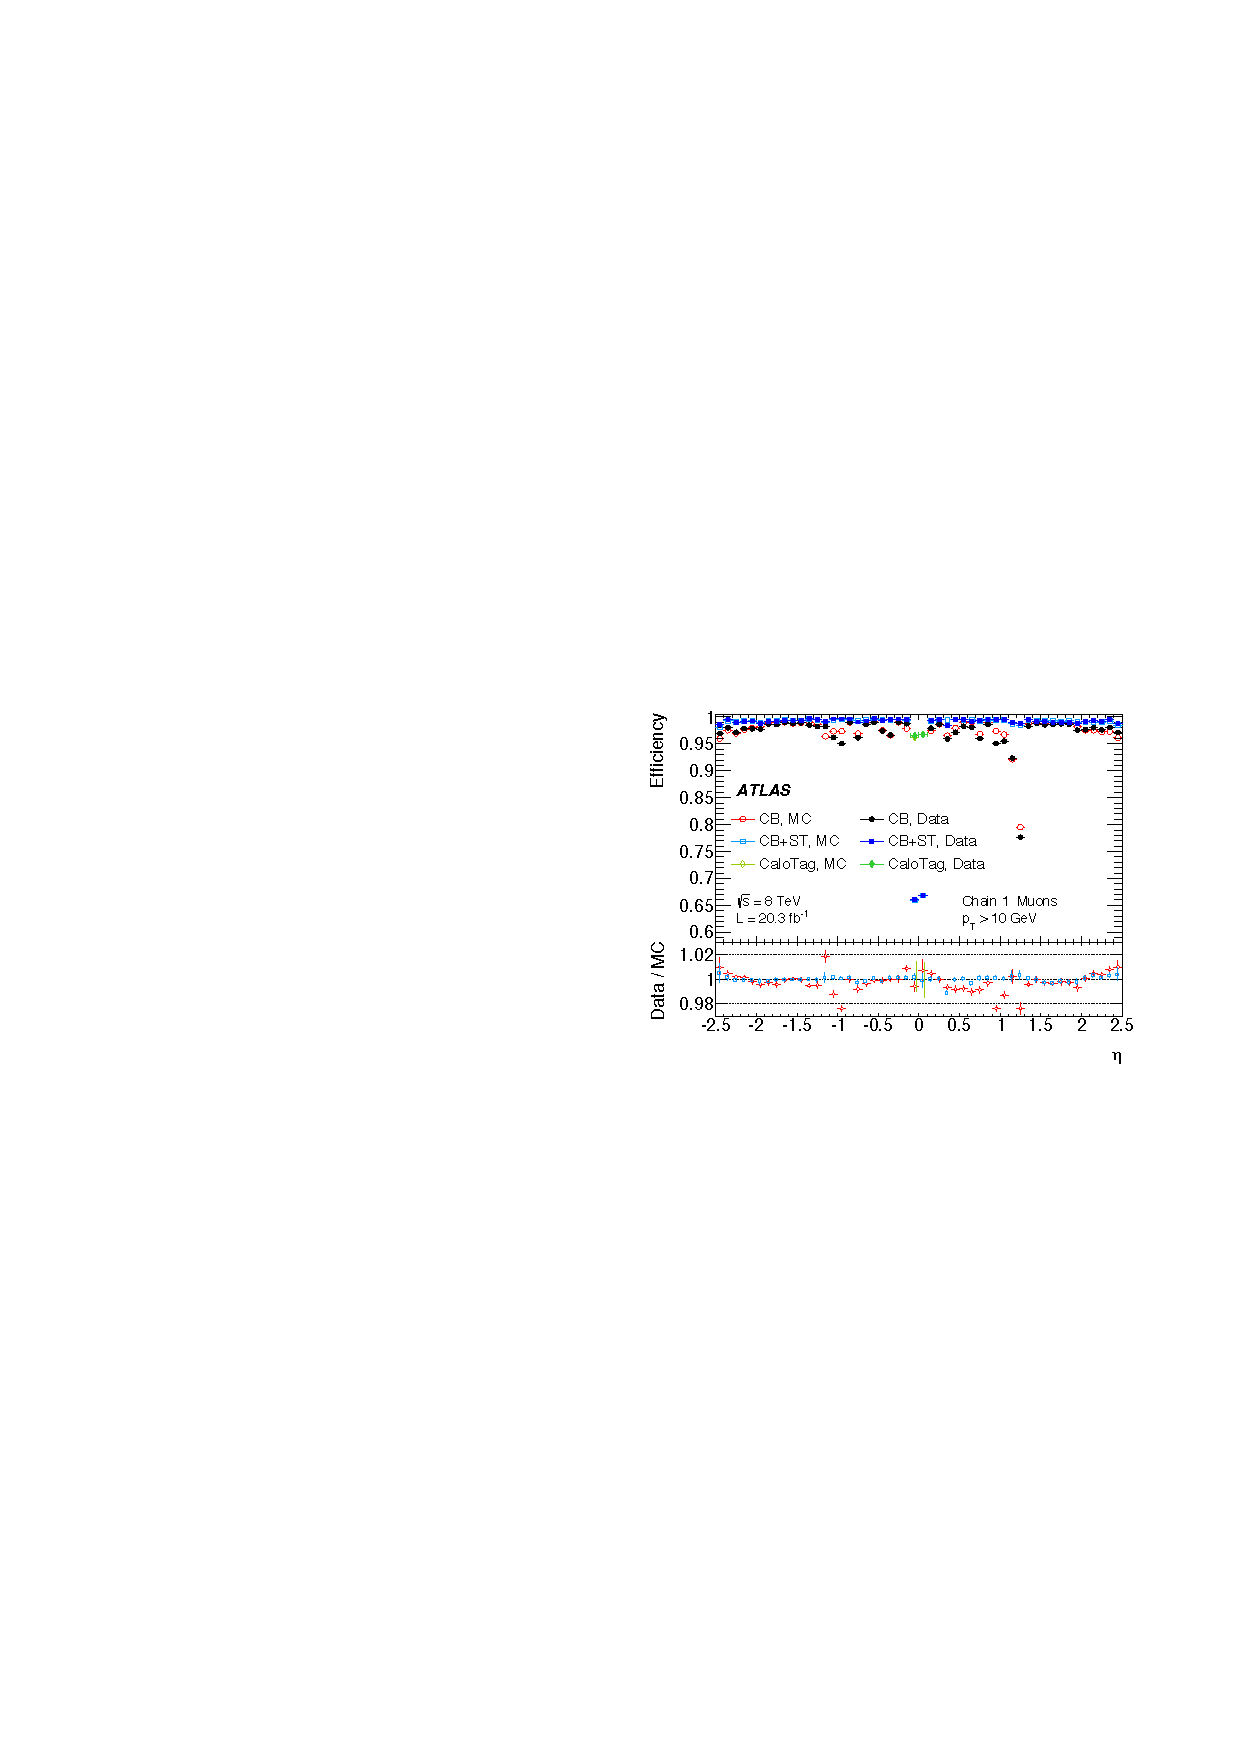
\includegraphics[width=0.48\textwidth]{figures/performance/muon-efficiency}
  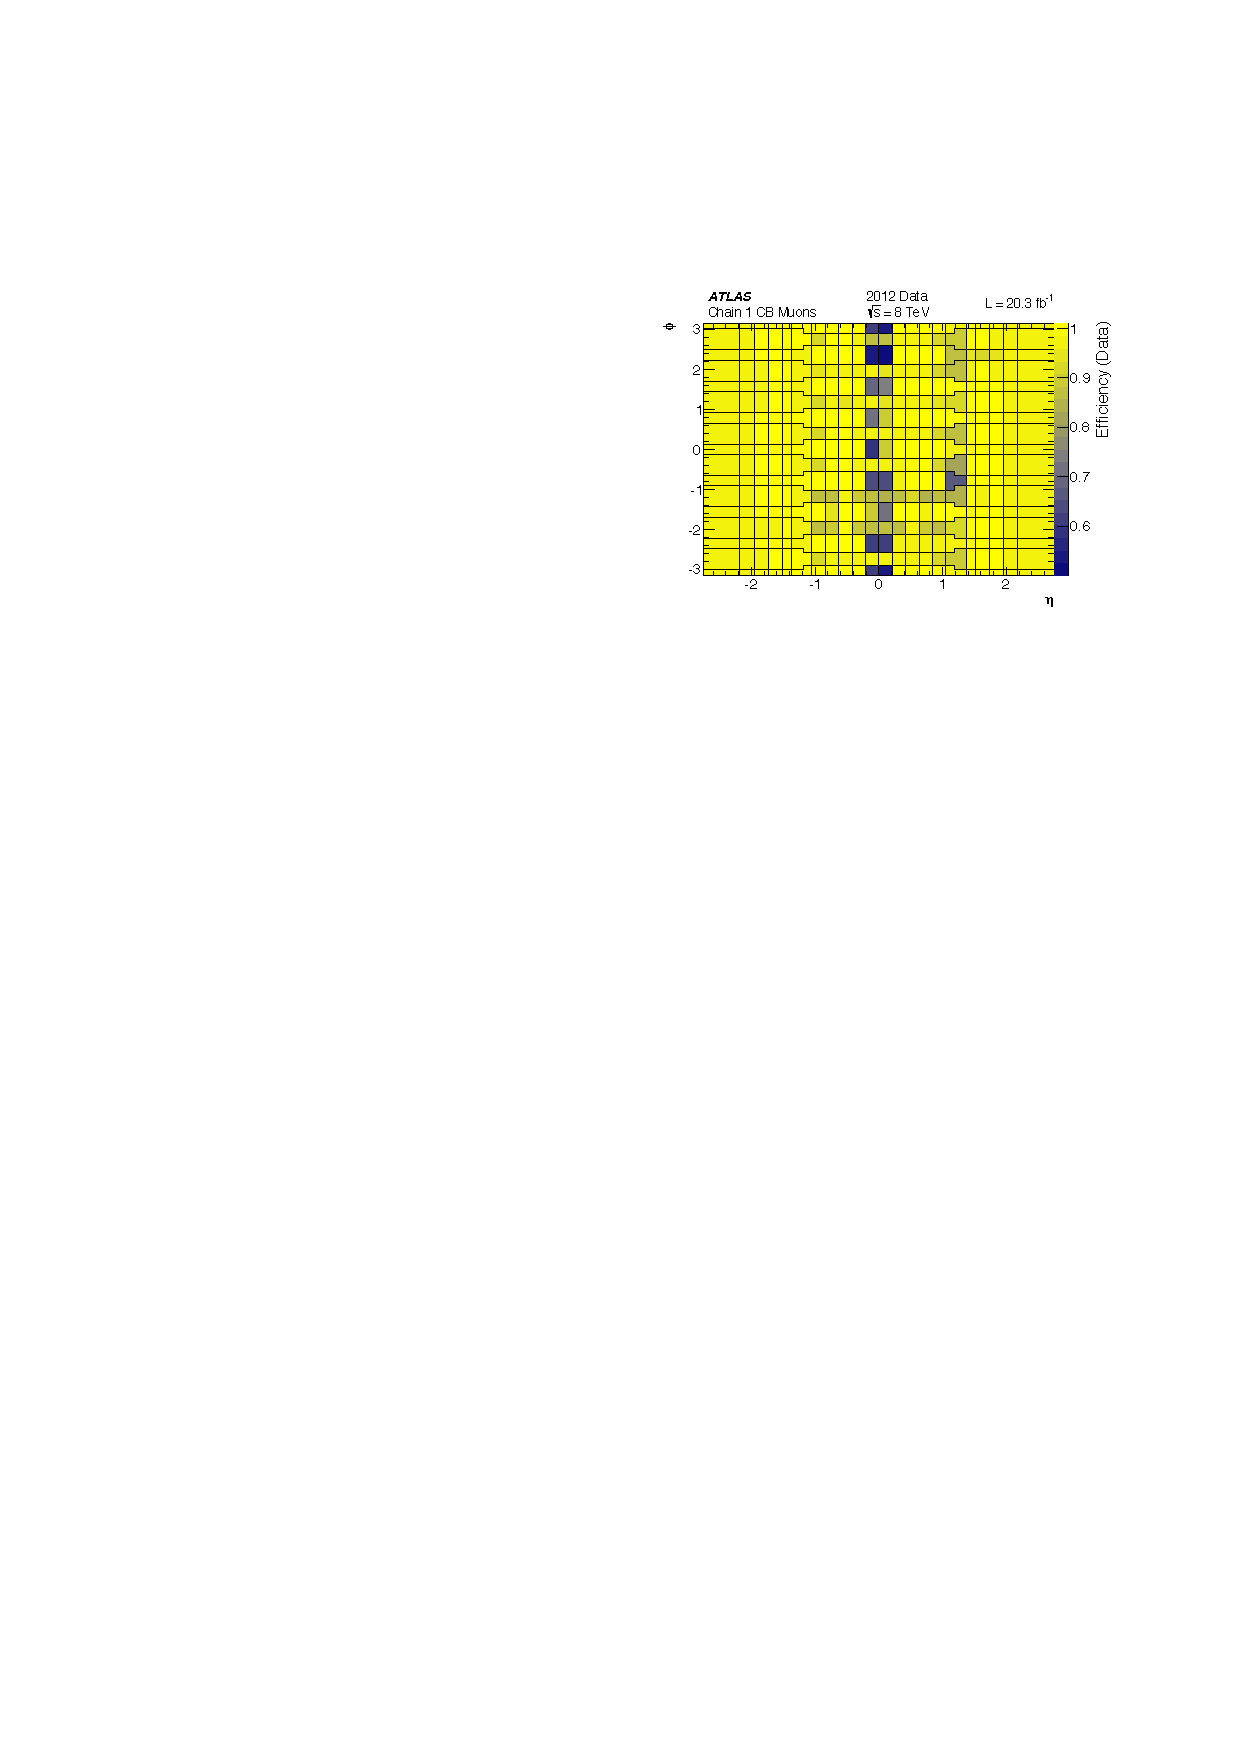
\includegraphics[width=0.48\textwidth]{figures/performance/muon-efficiency-etaphi}
  \caption{Measurement of the efficiency of the muon reconstructions algorithms in data and in simulation~\cite{PERF-2014-05}.}
  \label{fig:objects-muon-efficiency}
\end{figure}
\begin{figure}[tp]
  \centering
  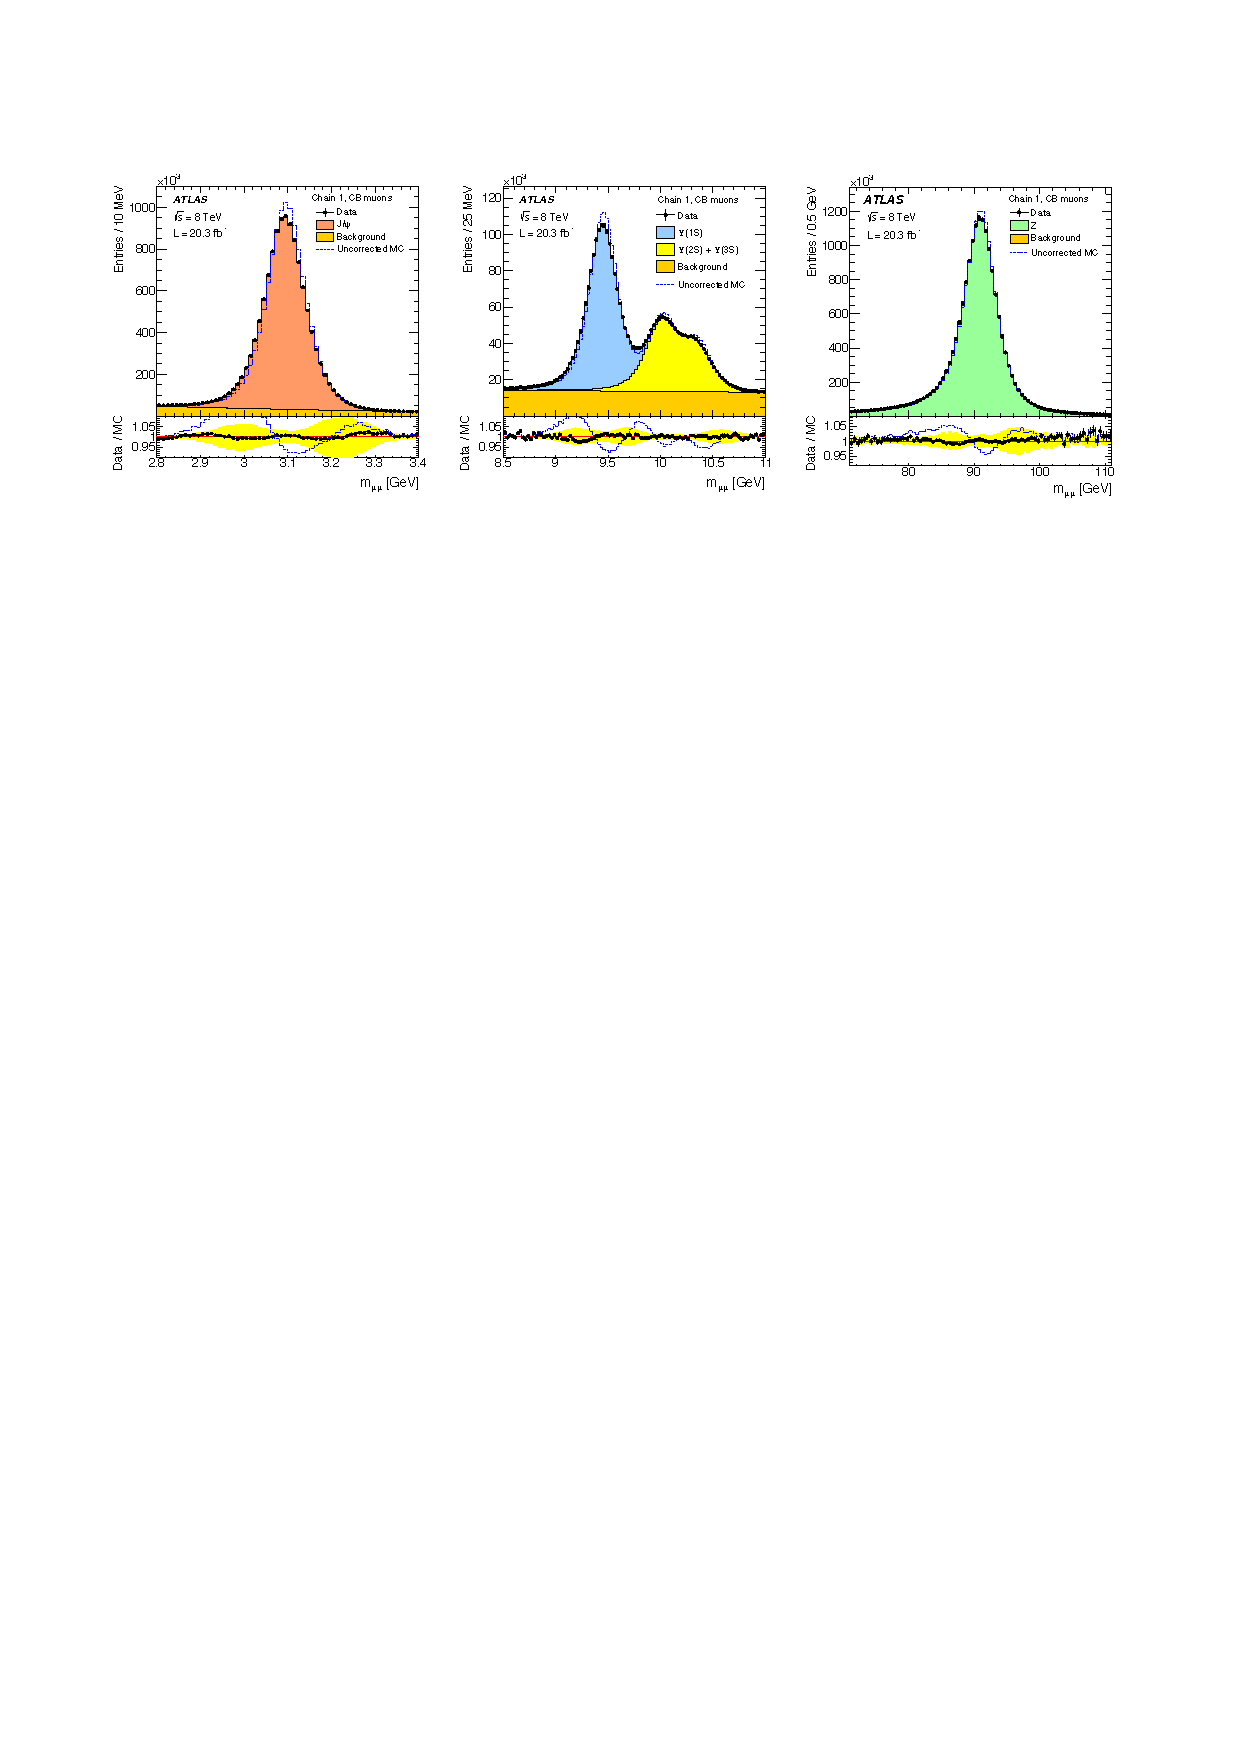
\includegraphics[width=0.90\textwidth]{figures/performance/muon-energyscale}
  \caption{Validation of the muon energy scale corrections in $J/\Psi$ events (left), $\Upsilon$ events (center), and $Z$ events (right)~\cite{PERF-2014-05}.}
  \label{fig:objects-muon-energyscale}
\end{figure}

\subsection{Electrons and photons}

\begin{figure}[tp]
  \centering
  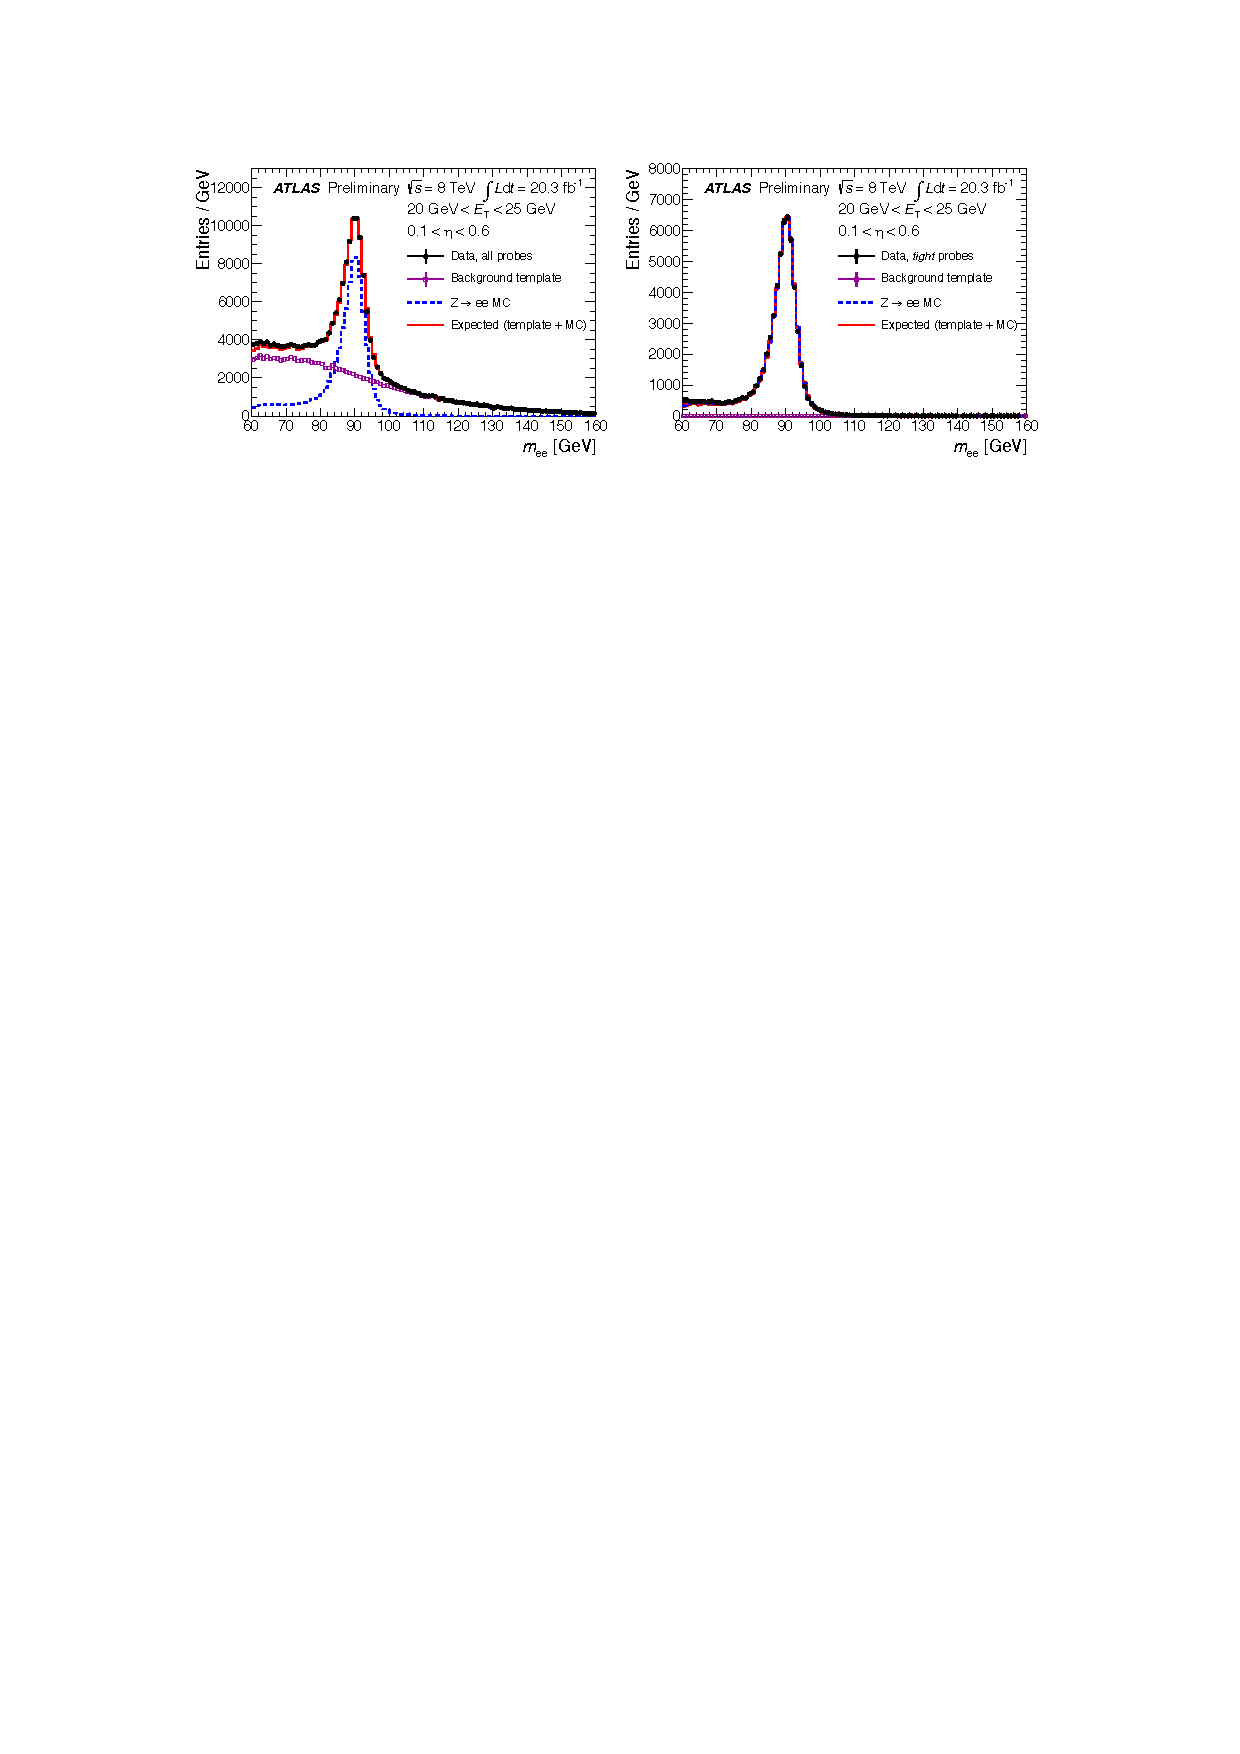
\includegraphics[width=0.90\textwidth]{figures/performance/electron-ZeeTP}
  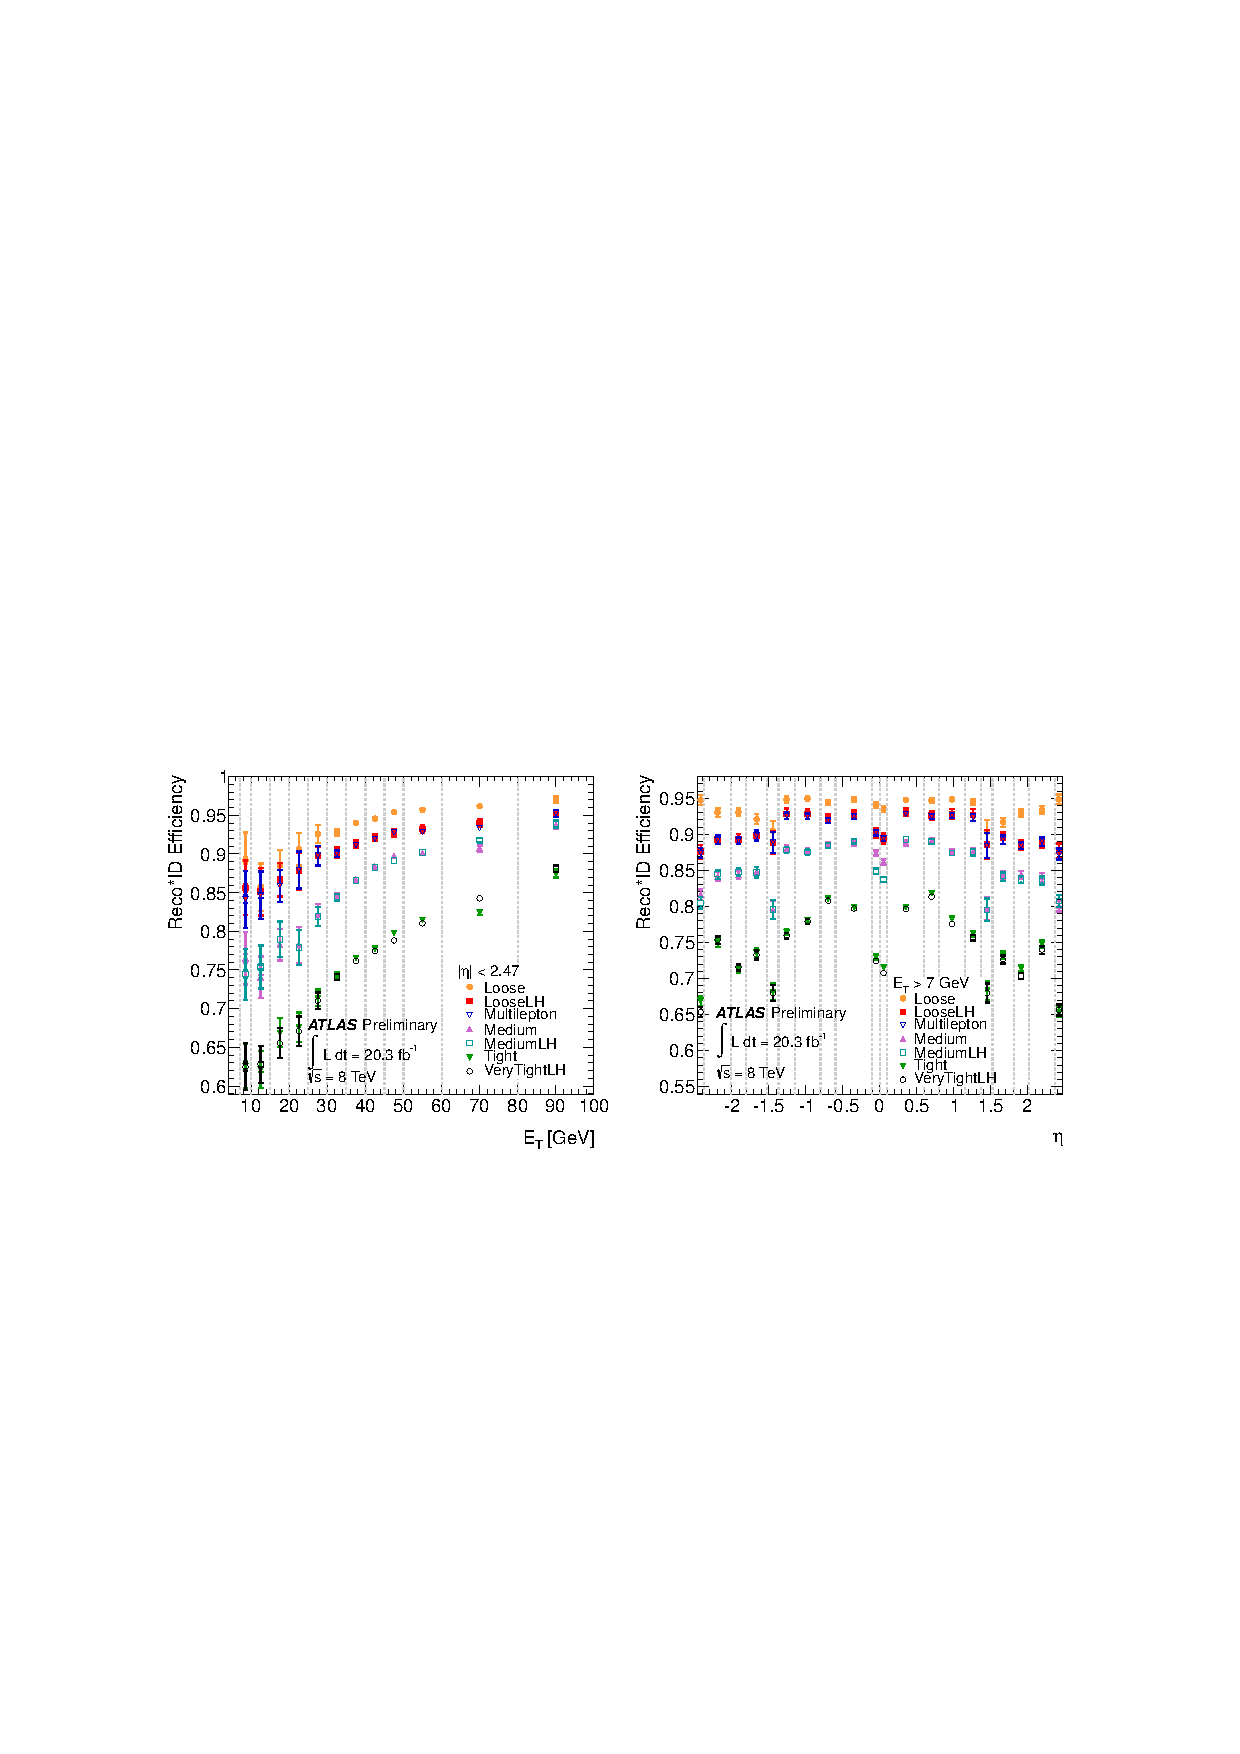
\includegraphics[width=0.90\textwidth]{figures/performance/electron-recoIDefficiecy}
  \caption{Data and predictions of $m_{ee}$ before the electron identification algorithm is applied (top, left) and after (top, right), and the measured efficiency of the algorithm as a function of $\text{E}_\text{T}$ (bottom, left) and $\eta$ (bottom, right)~\cite{ATLAS-CONF-2014-032}.}
  \label{fig:objects-electron}
\end{figure}

\subsection{Hadrons}

\begin{figure}[tp]
  \centering
  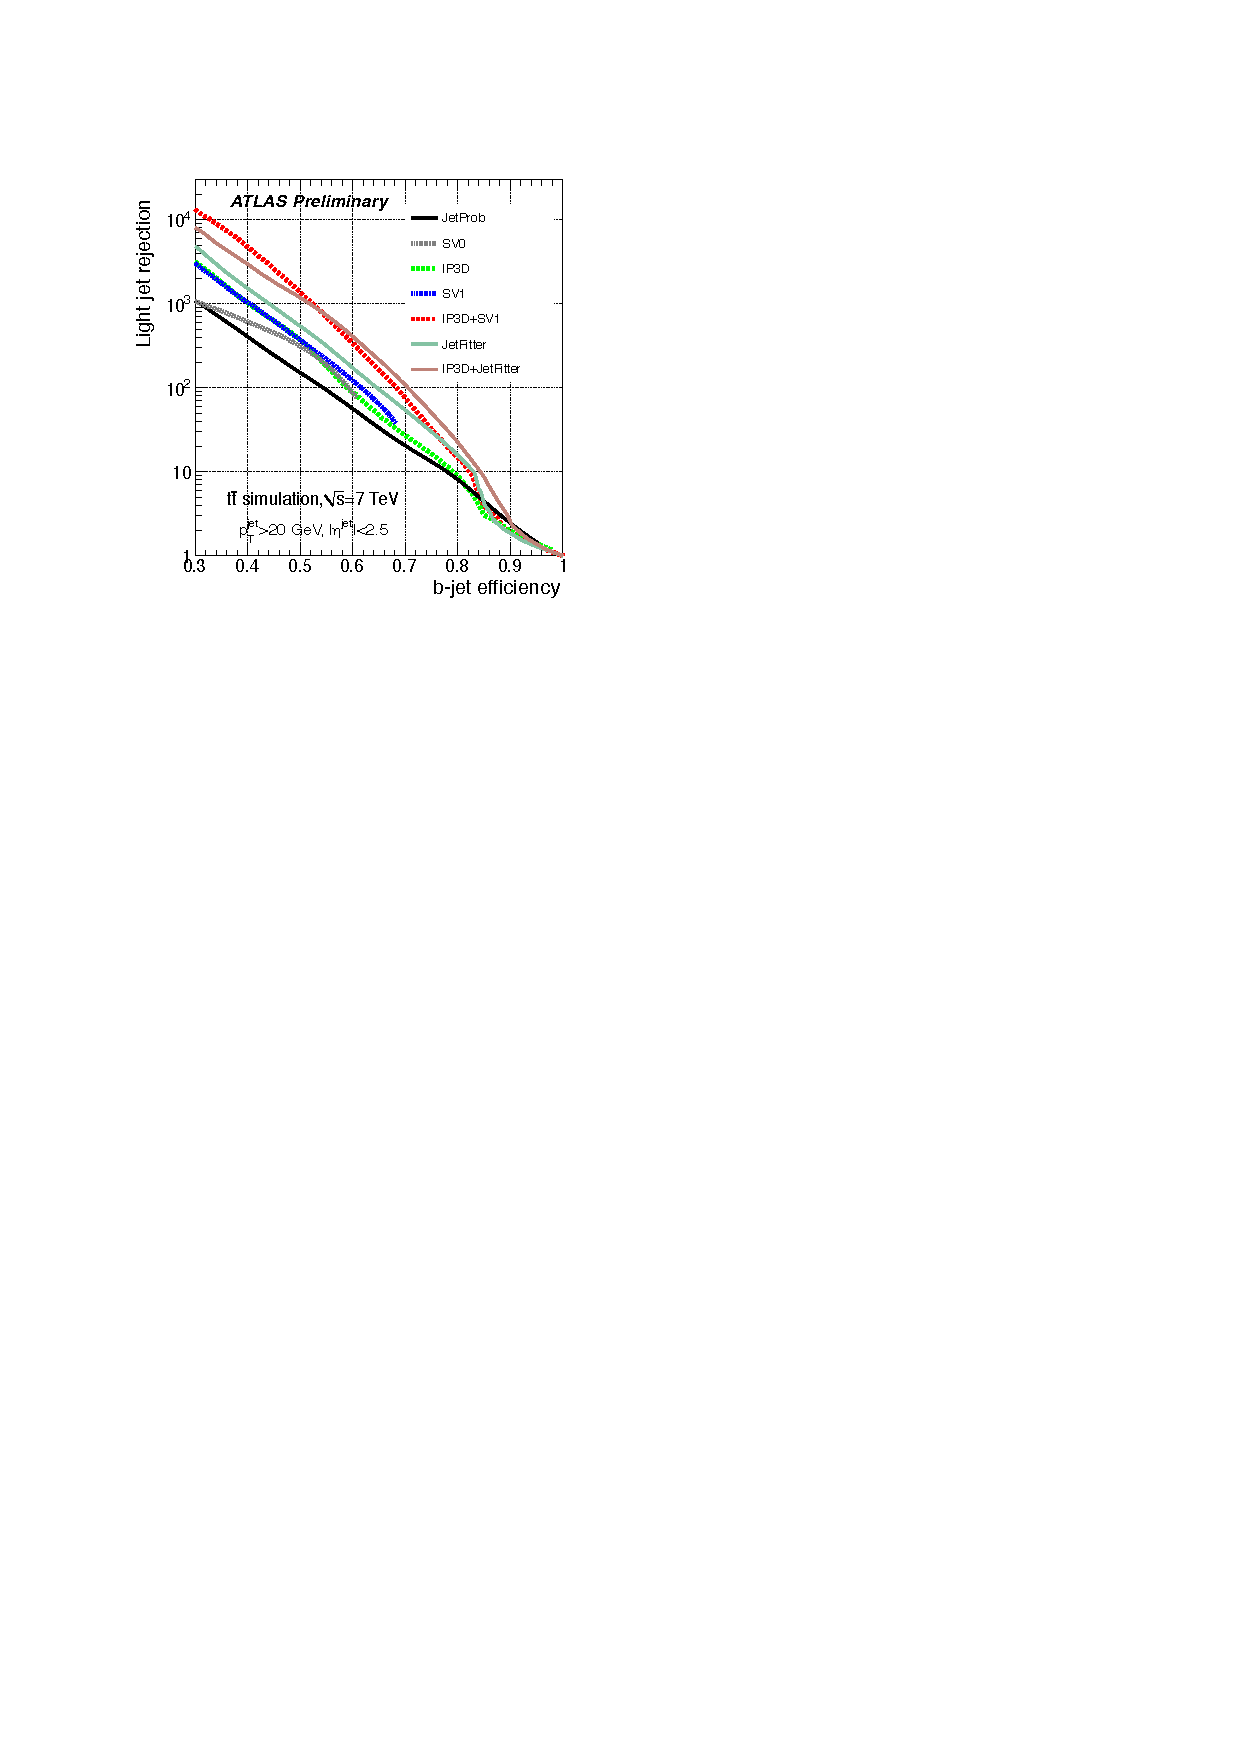
\includegraphics[width=0.48\textwidth]{figures/performance/btag-ROC}
  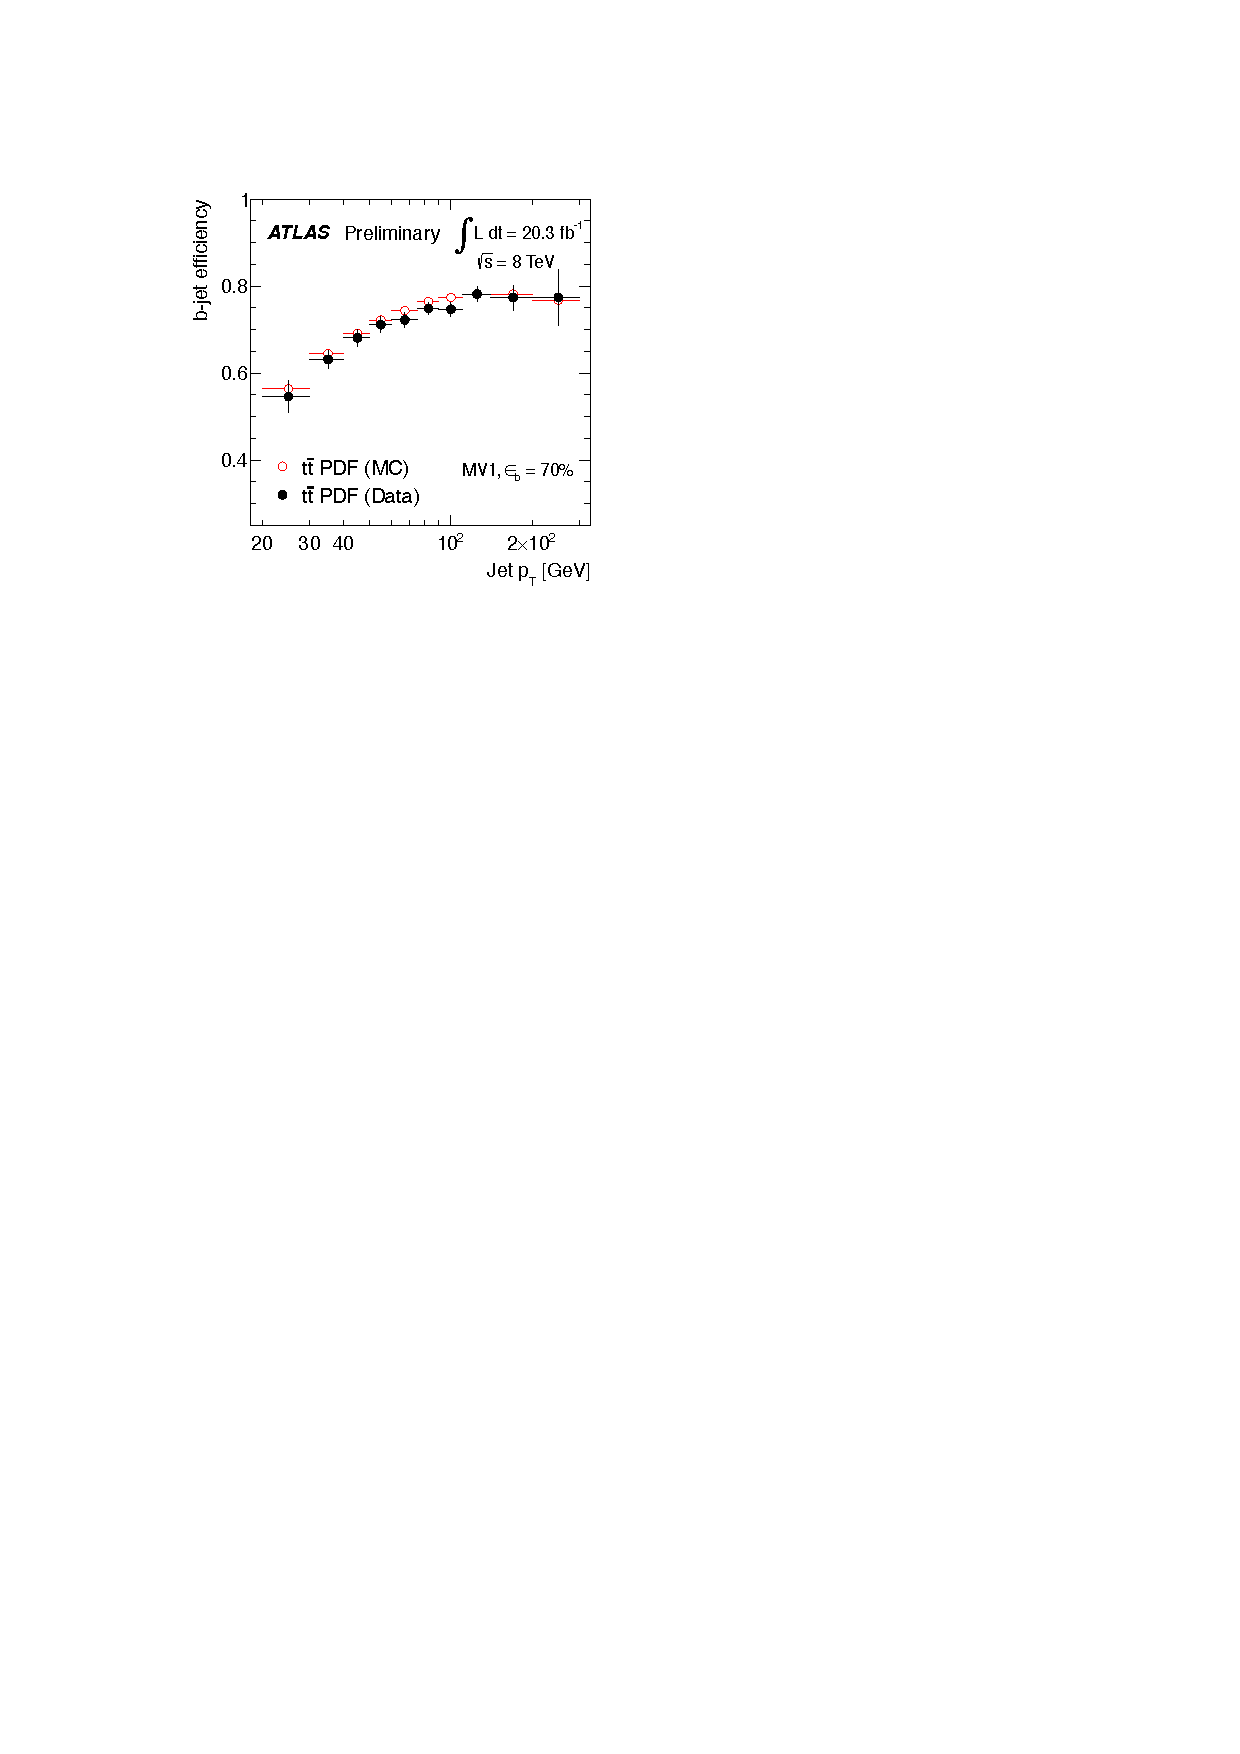
\includegraphics[width=0.48\textwidth]{figures/performance/btag-signalefficiency}
  \caption{Efficiency of $b$-jet identification algorithms measured in simulation as a function of light jet rejection (left)~\cite{ATLAS-CONF-2012-043} and $b$-jet $\pt$ (right)~\cite{ATLAS-CONF-2014-004}.}
  \label{fig:objects-btag}
\end{figure}

\subsection{Neutrinos}

\begin{figure}[tp]
  \centering
  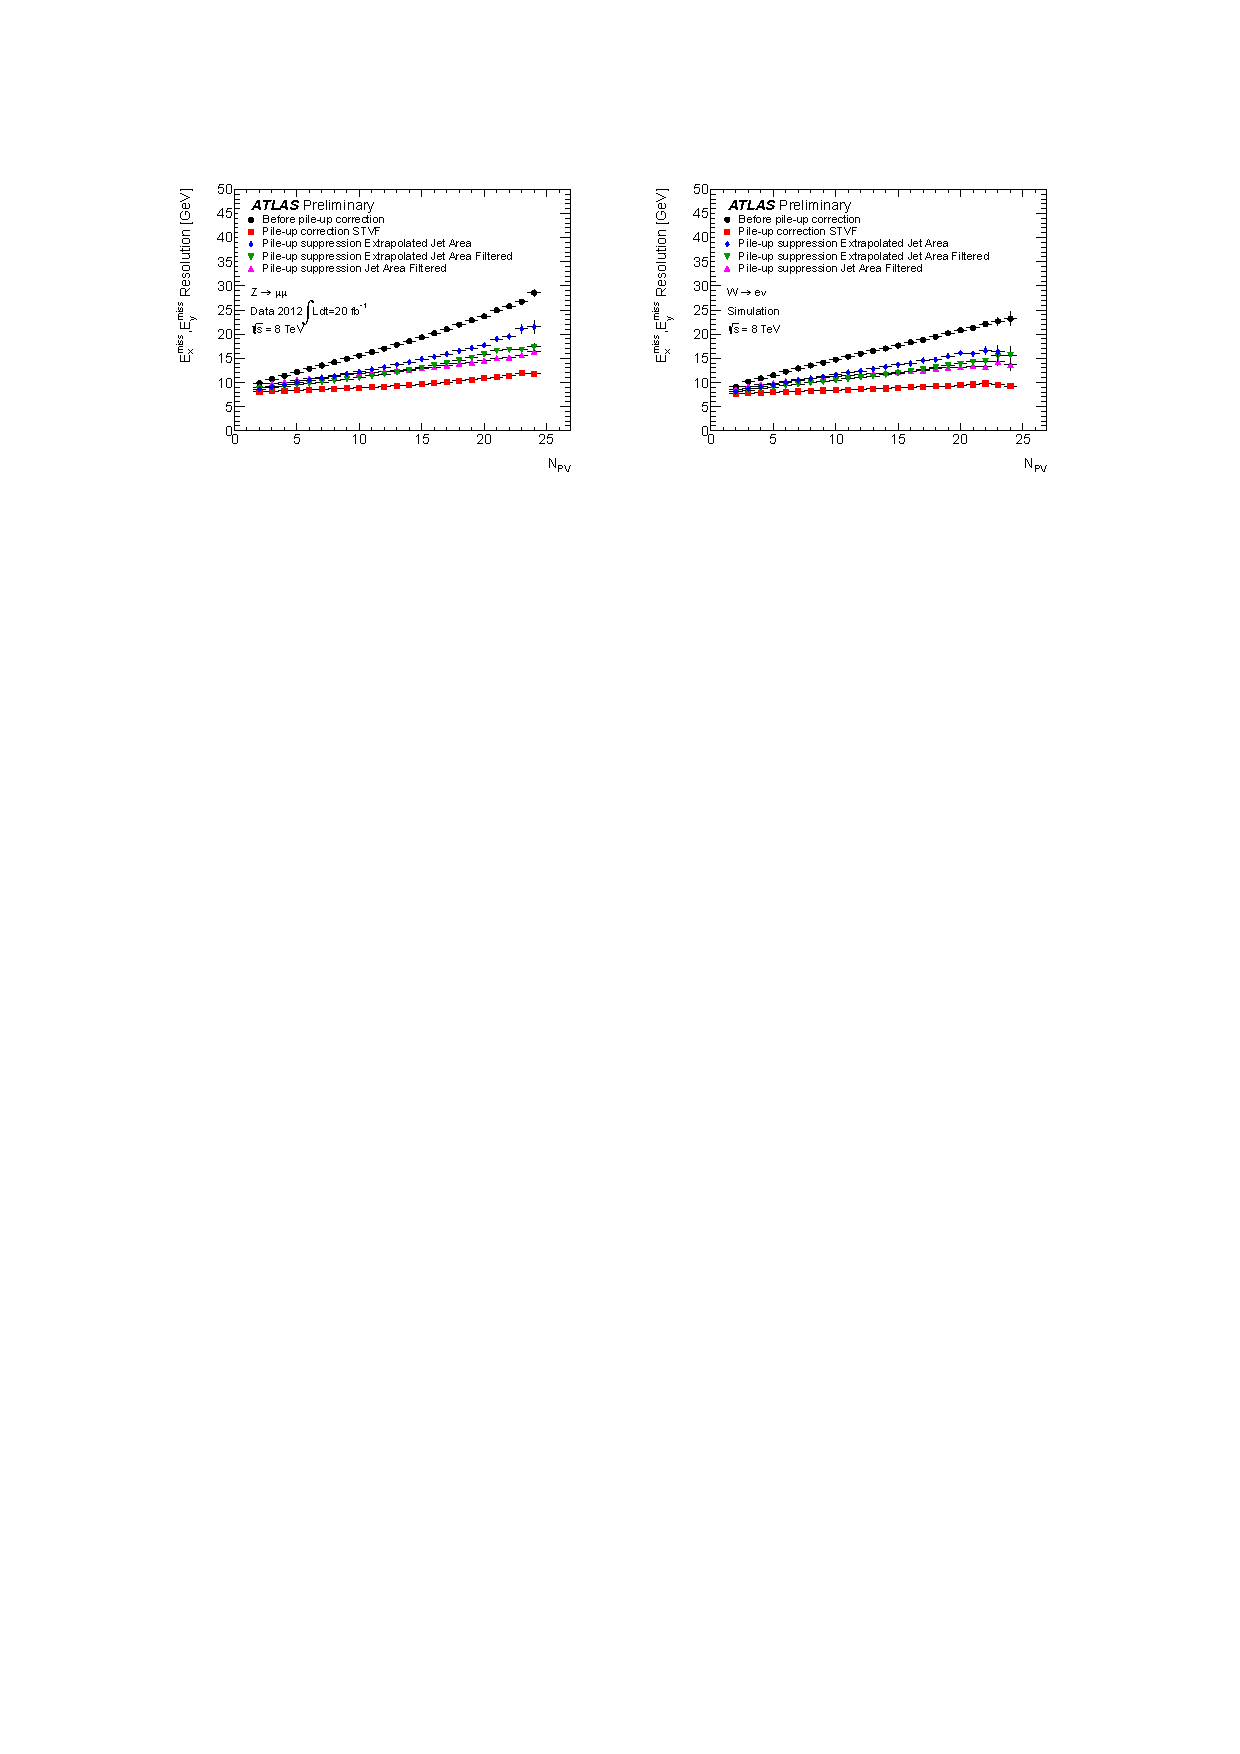
\includegraphics[width=0.90\textwidth]{figures/performance/met-resolutionvsnpv}
  \caption{Resolution of various $\MET$ reconstruction algorithms as a function of the number of reconstructed primary vertices in $\Zmm$ events in data (left) and $\Wen$ events in simulation (right)~\cite{ATLAS-CONF-2014-019}.}
  \label{fig:objects-met-resolution}
\end{figure}
\begin{figure}[tp]
  \centering
  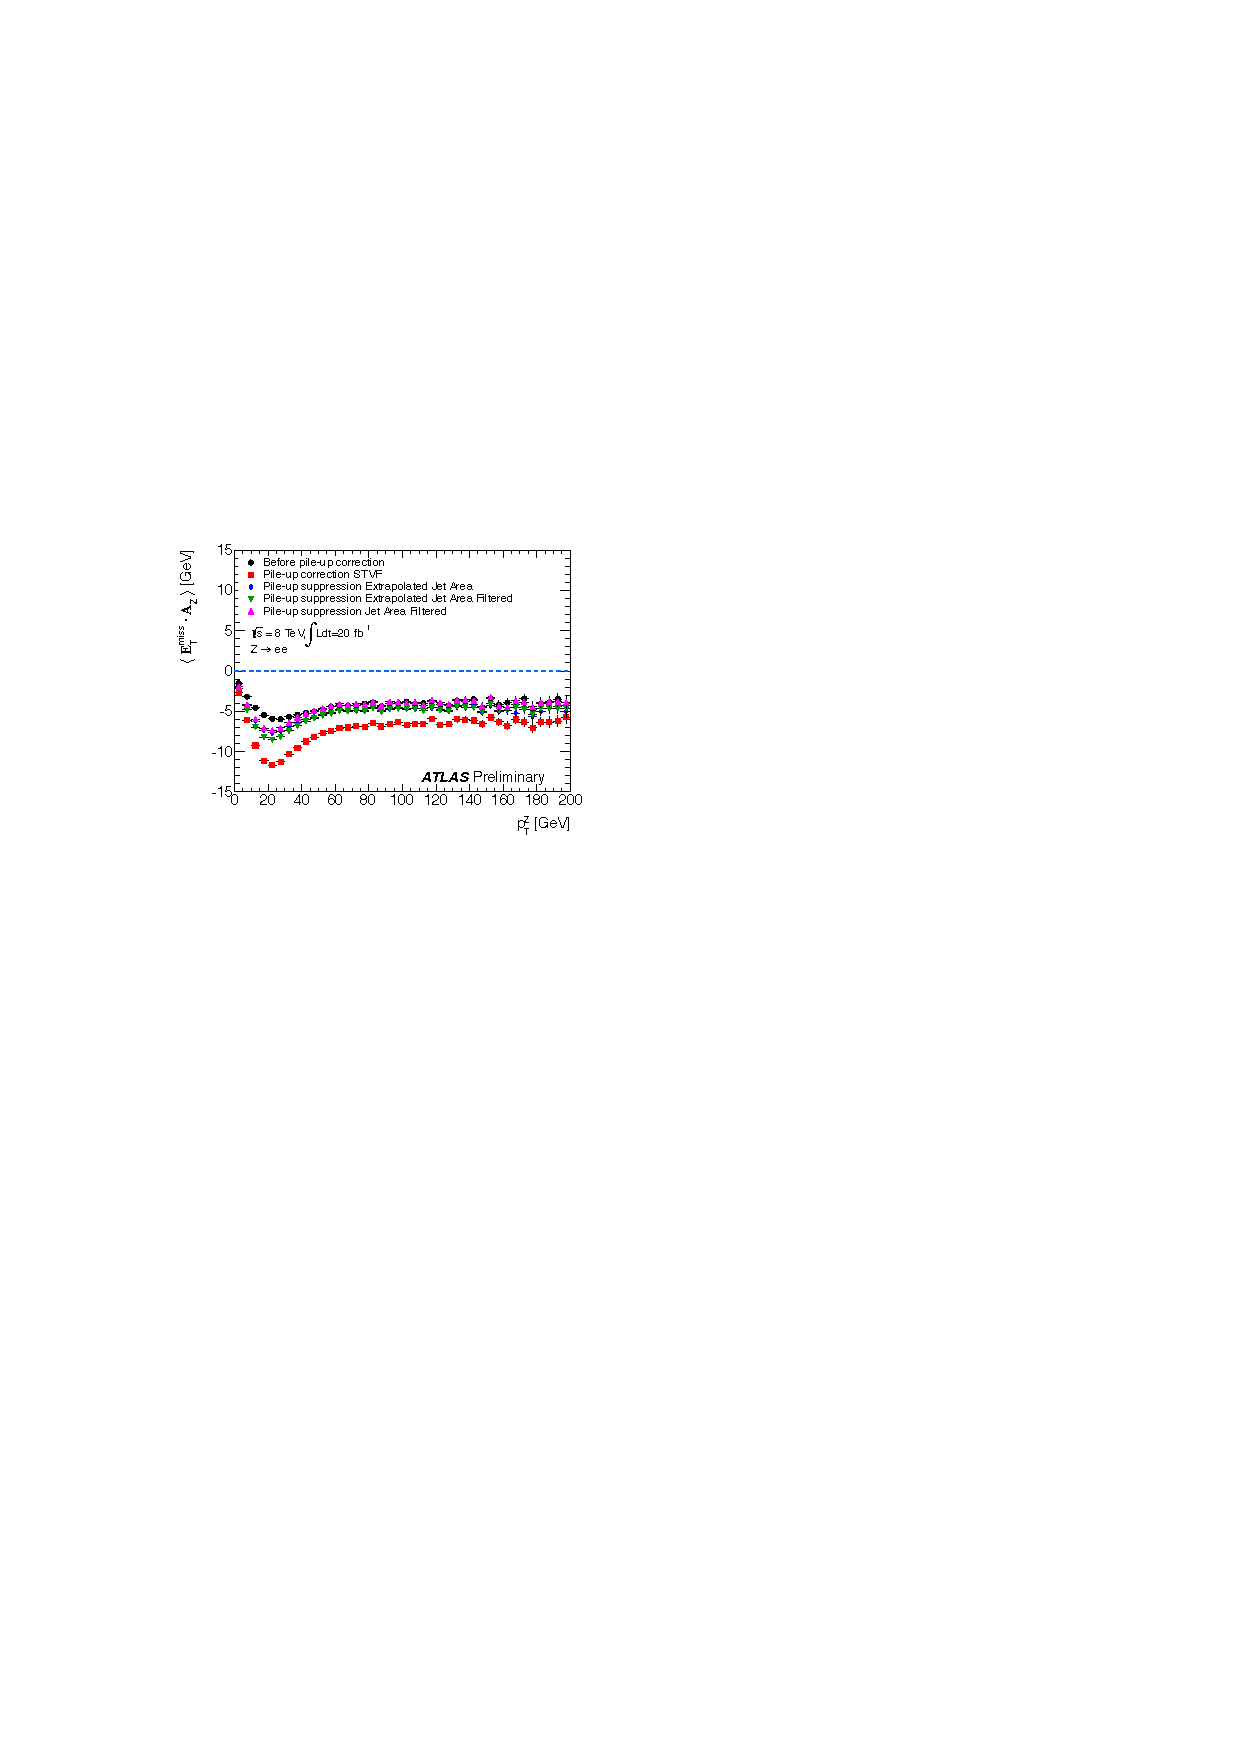
\includegraphics[width=0.48\textwidth]{figures/performance/met-bias-inclusive}
  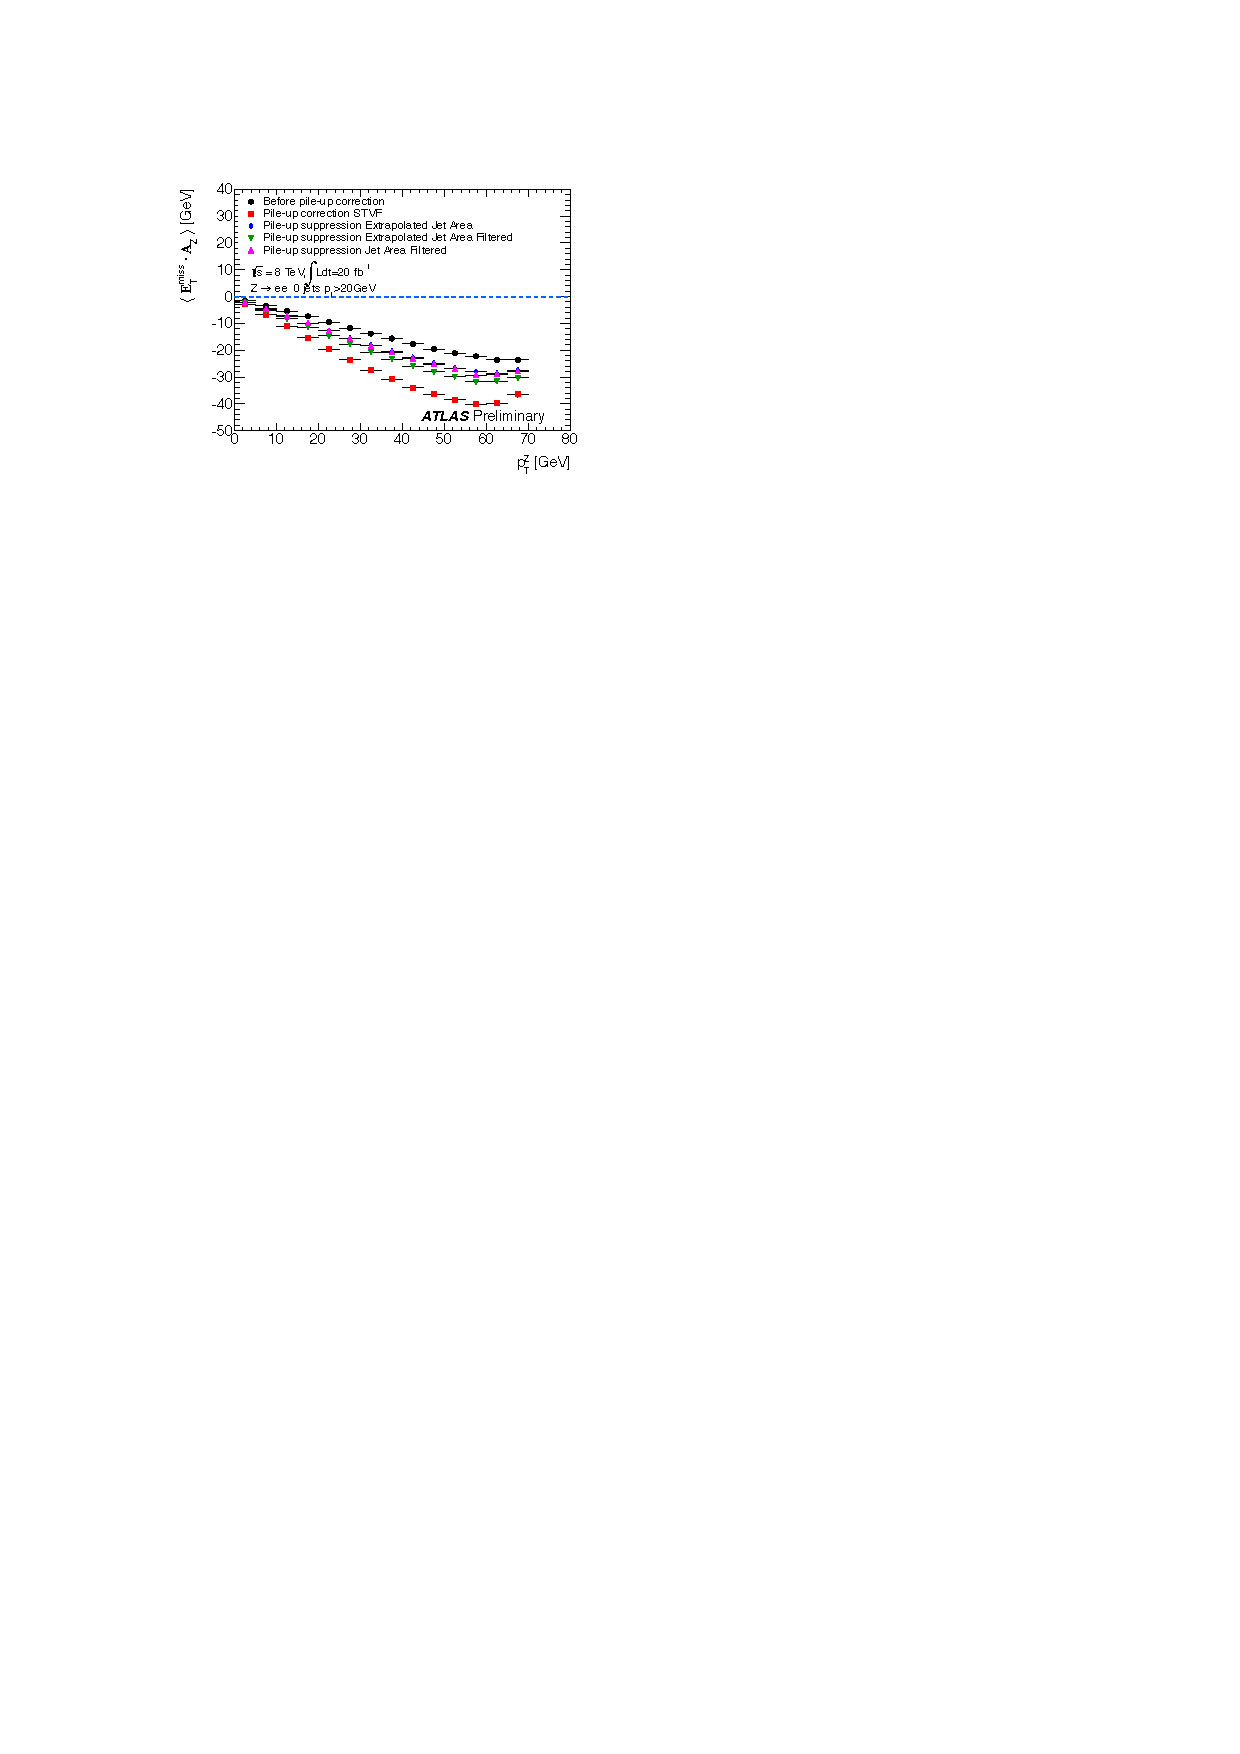
\includegraphics[width=0.48\textwidth]{figures/performance/met-bias-0jet}
  \caption{Bias of various $\MET$ reconstruction algorithms as a function of $\pt^Z$ measured in data events inclusively (left) and with no additional jets (right)~\cite{ATLAS-CONF-2014-019}.}
  \label{fig:objects-met-bias}
\end{figure}

\section{Triggering}

One of the most challenging aspects of physics at hadron colliders is that the vast majority of $pp$ collisions produce low $\pt$ QCD dijets which are mostly uninteresting in searches for new physics.

\subsection{L1}
\subsection{HLT}


\begin{figure}[tp]
  \centering
  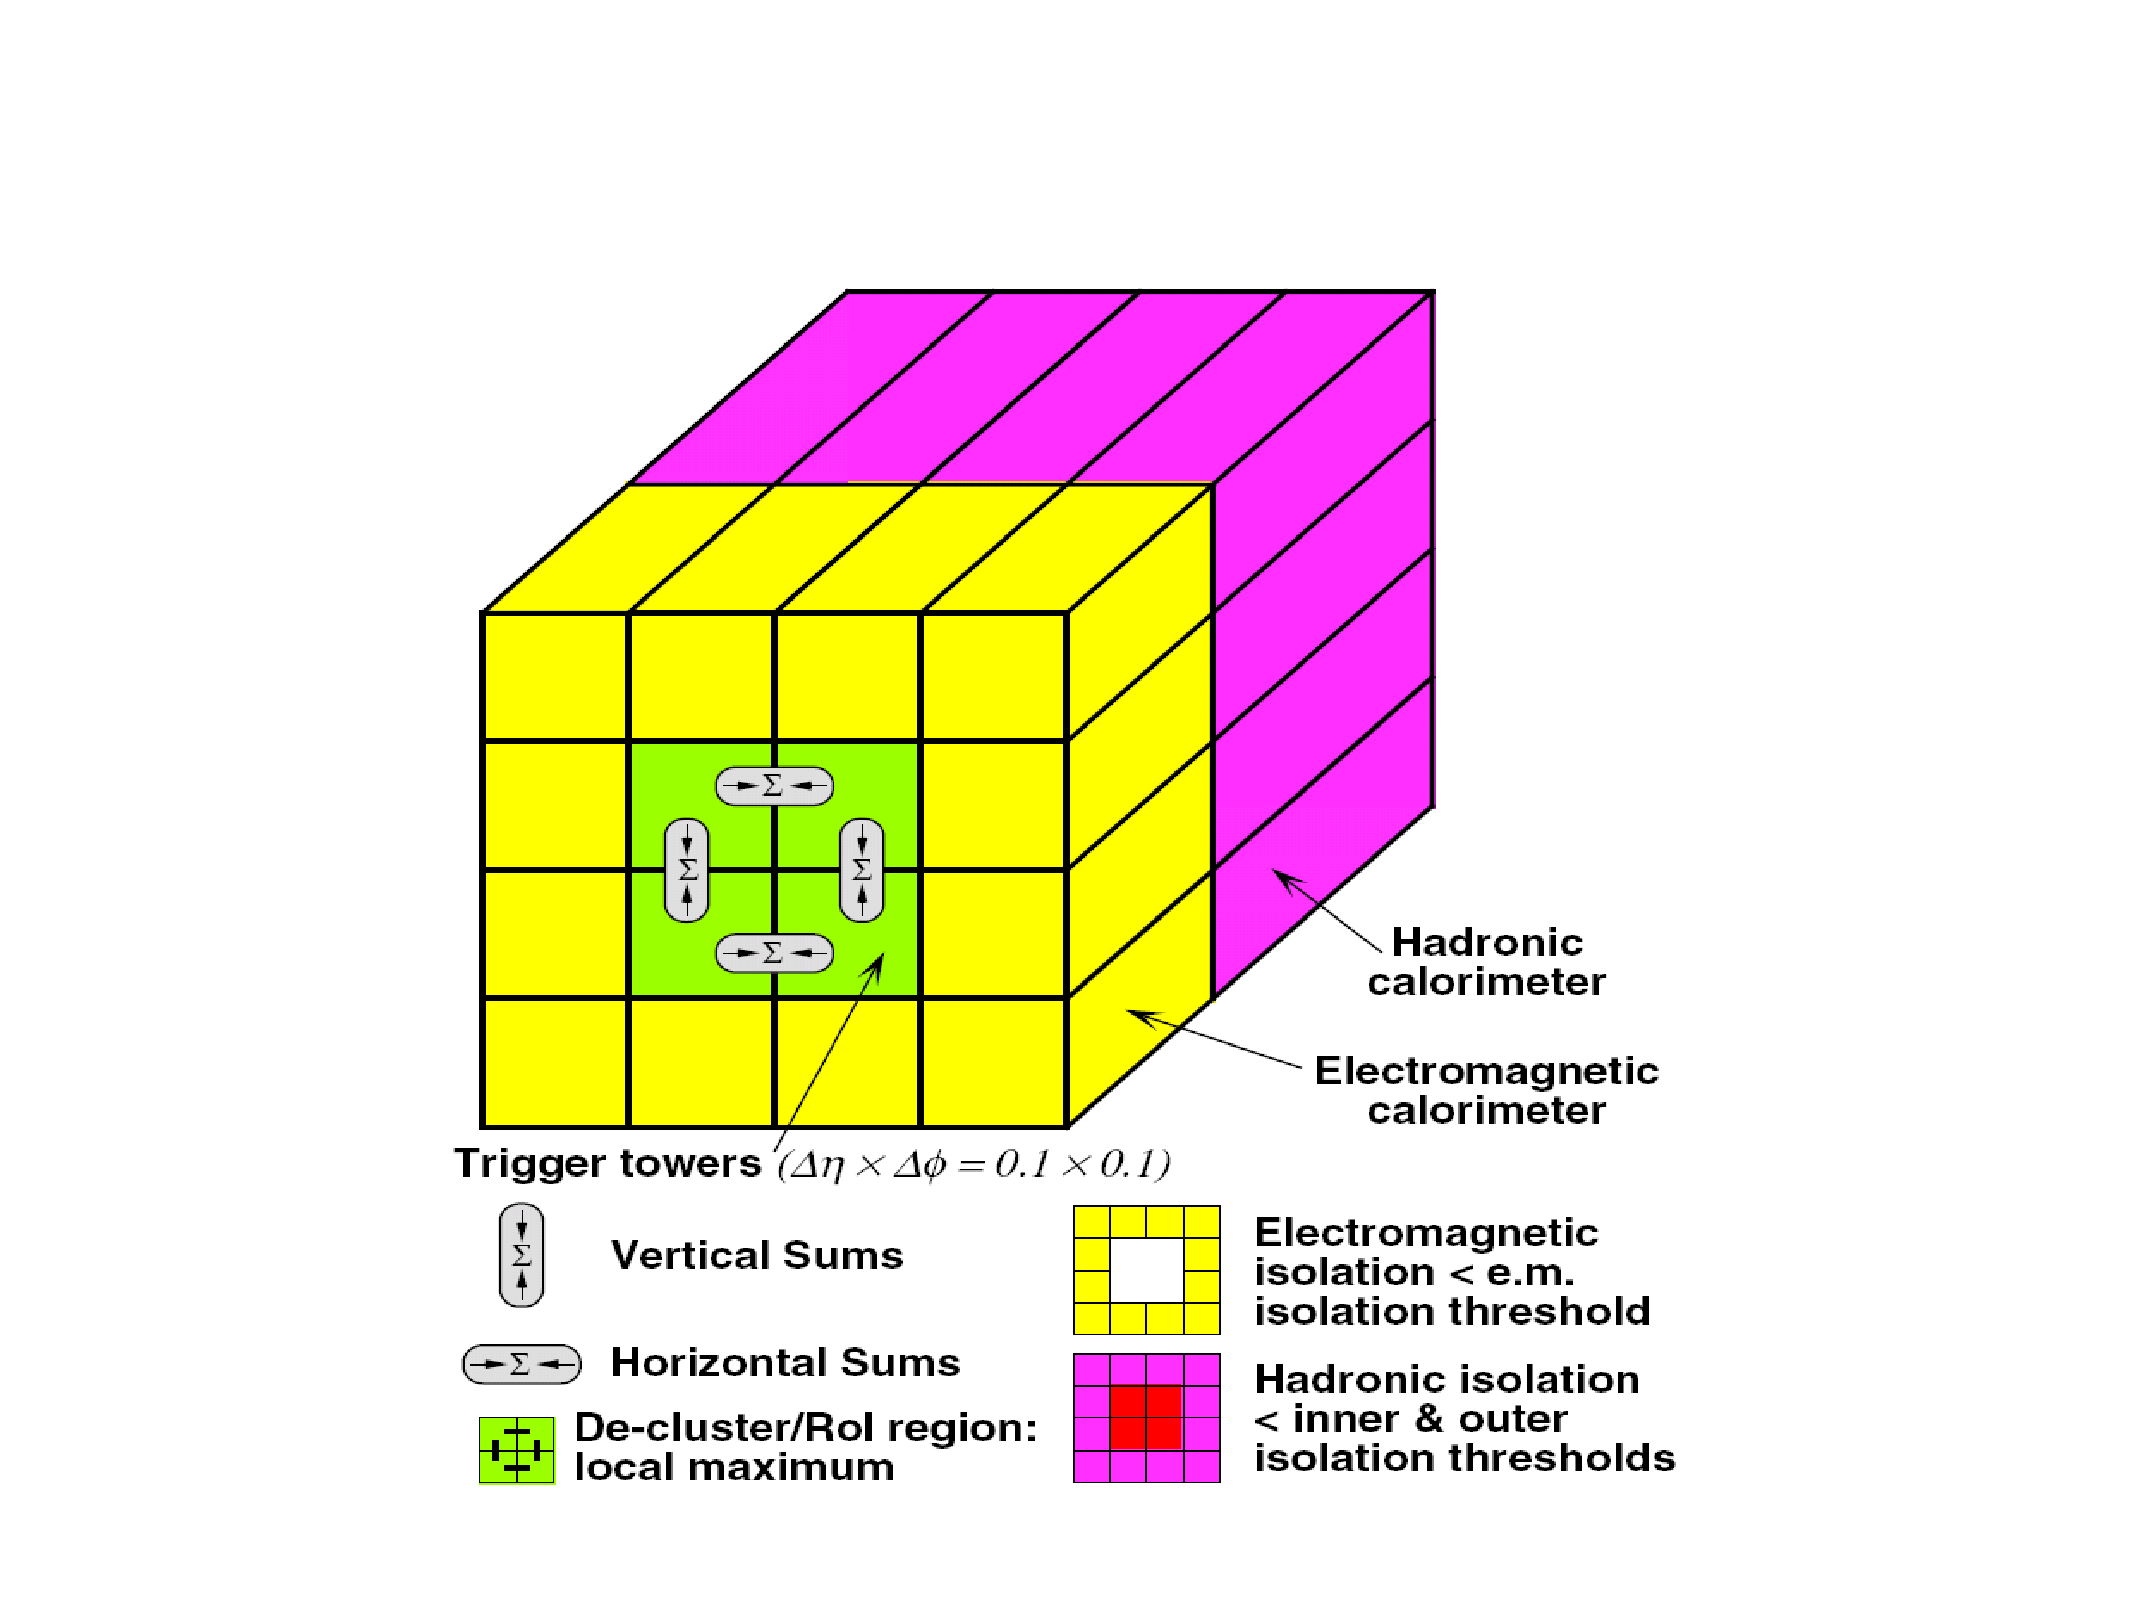
\includegraphics[width=0.80\textwidth]{figures/trigger/cartoonL1}
  \caption{Schematic view of the calorimeter granularity available at the L1 trigger~\cite{1998.ATLAS-TDR-L1}.}
  \label{fig:prospects-trigger-cartoonL1}
\end{figure}

\begin{figure}[tp]
  \centering
  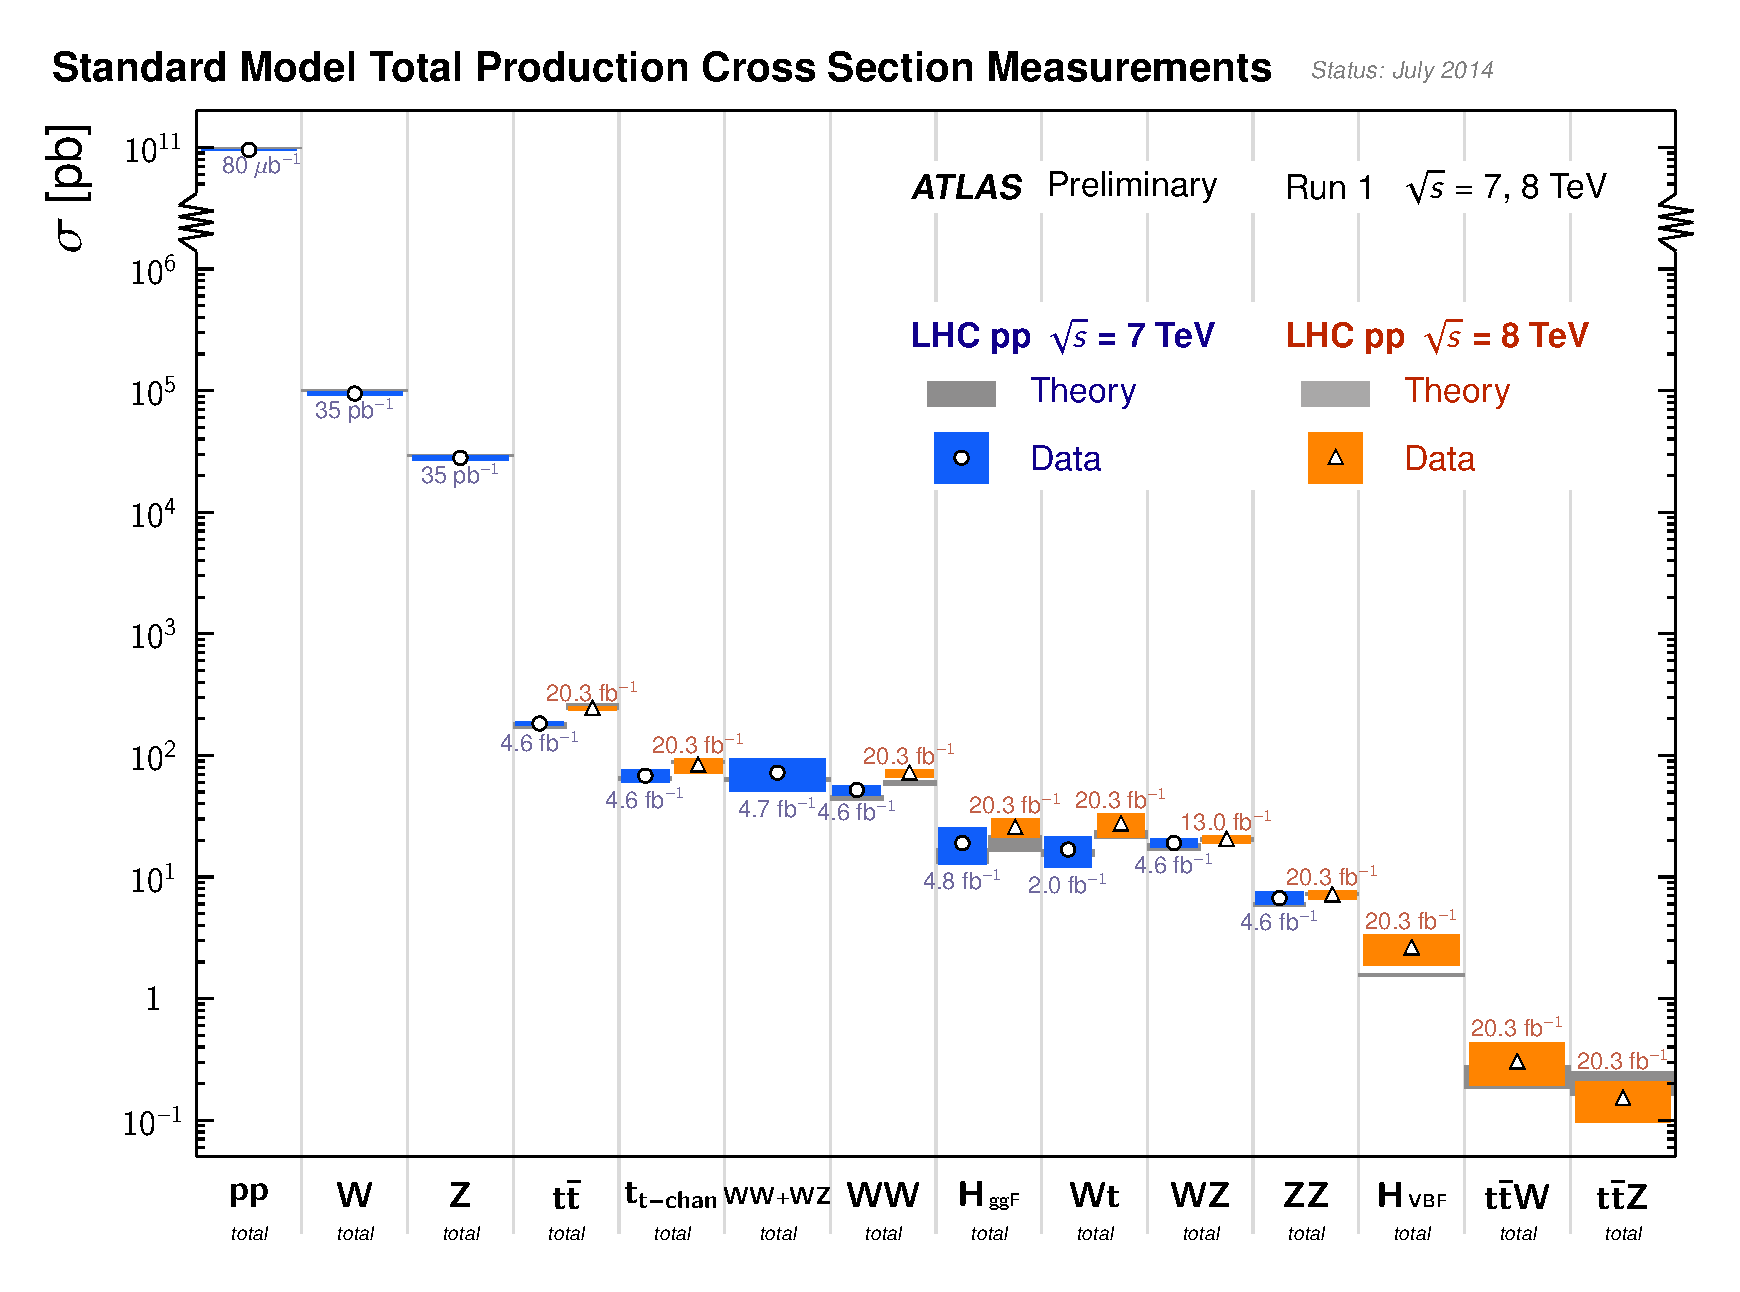
\includegraphics[width=0.90\textwidth]{figures/lhc-atlas/ATLAS_a_SMSummary_TotalXsect}
  \caption{Summary of cross sections measured at ATLAS in 7 and 8 TeV data-taking~\cite{2015.atlas-summary-SM}.}
  \label{fig:atlas-measurements}
\end{figure}


